\documentclass[a4paper, 10pt]{article}

\usepackage{graphicx}
\graphicspath{ {./docassets} }
\usepackage{float} % add `H` floating parameter so figures appear like I want
\usepackage{tcolorbox}

% reduce space between images and captions
\usepackage{caption}
\captionsetup{skip=8pt, belowskip=-8pt}

% code highlighting
\usepackage{minted}
\usepackage[svgnames]{xcolor}

\setminted{
  autogobble,
  style=vs,
  breaklines,
  frame=single,
  framesep=2mm,
  linenos,
  baselinestretch=1.05,
  fontsize=\small,
  numbersep=4pt,
  tabsize=2
}

\renewcommand{\theFancyVerbLine}{ % customize line numbers
  \ttfamily
  \textcolor[rgb]{0.2,0.2,0.2}{
    \footnotesize
      \arabic{FancyVerbLine}}}

% requirements for work formatting
% 2.5cm edge for pages
\usepackage[margin=2.5cm]{geometry}
% use Helvetica as default font (unfortunately no required Verdana)
\usepackage[T1]{fontenc}
\usepackage{helvet}
\renewcommand{\familydefault}{\sfdefault}
% use inconsolata for monoscape font
\usepackage{textcomp}
\usepackage[scaled]{inconsolata}
% line spacing of 1.5
\usepackage{setspace}
\onehalfspacing
% paragraph spacing of 12 points
\setlength{\parskip}{12pt}
\setlength{\parindent}{0pt} % remove indent at the start of paragraph
% place page numbers on the right
\usepackage{fancyhdr}
\pagestyle{fancy}
\fancyhf{} % clear existing header/footer
\fancyfoot[R]{\thepage} % put page number on the right
\renewcommand{\headrulewidth}{0pt} % remove header line

% format sections by the work format requirements
\usepackage{titlesec}
% section (14pt, uppercase, 12pt spacing)
\titleformat{\section}
  {\bfseries\fontsize{14pt}{16pt}\selectfont}
  {\thesection}{1em}{\MakeUppercase}
\titlespacing*{\section}{0pt}{12pt}{12pt}
% subsction (12pt, uppercase, 12pt spacing)
\titleformat{\subsection}
  {\bfseries\fontsize{12pt}{14pt}\selectfont}
  {\thesubsection}{1em}{\MakeUppercase}
\titlespacing*{\subsection}{0pt}{12pt}{12pt}
% subsubsection (10pt, uppercase, 12pt spacing)
\titleformat{\subsubsection}
  {\bfseries\fontsize{10pt}{12pt}\selectfont}
  {\thesubsubsection}{1em}{\MakeUppercase}
\titlespacing*{\subsubsection}{0pt}{12pt}{12pt}

% remove \parskip from the table of contets
\makeatletter
\patchcmd{\tableofcontents}
  {\@starttoc{toc}}
  {\begingroup
   \setlength{\parskip}{0pt}
   \@starttoc{toc}
   \endgroup}
  {}{}
\makeatother

% must be loaded after all packages
\usepackage[
  colorlinks=true,
  linkcolor=blue!50!black,
  urlcolor=blue!70!black,
  citecolor=green!40!black,
  pdfborder={0 0 0},
  breaklinks=true
]{hyperref}
\usepackage{xurl}

% add page break before each section
\let\oldsection\section
\renewcommand{\section}{
  \clearpage
  \oldsection
}

% For estonian
\renewcommand{\contentsname}{Sisukord}
\renewcommand{\figurename}{Joonis}

\newcommand{\theauthor}{Retro }
\newcommand{\theteacher}{Õpetaja }


\begin{document}

\sloppy

\begin{center}
  \Large
  TALLINNA POLÜTEHNIKUM \\
  IT ja telekommunikatsiooni erialaosakond

  \vspace*{\fill}

  \theauthor

  {\huge P2P VPN-RAKENDUSE ARETAMINE}

  Lõputöö

  Tarkvaraarendaja \\
  TA-22V

  \vspace*{\fill}

  \begin{flushright}
    Juhendaja: \theteacher
  \end{flushright}

  \vspace{4em}

  Tallinn 2026

\end{center}
\thispagestyle{empty}

\section*{AUTORIDEKLARATSIOON}

\vspace{3em}

Deklareerin, et käesolev lõputöö, mis on minu iseseisva töö tulemus, on esitatud Tallinna
Polütehnikumi lõputunnistuse taotlemiseks Tarkvaraarendaja erialal. Lõputöö alusel ei ole
varem eriala lõputunnistust taotletud.

\vspace{4em}

Autor \theauthor \emph{<allkirjastatud digitaalselt>}

\vspace{4em}

Töö vastab kehtivatele nõuetele

\vspace{4em}

Juhendaja \theteacher \emph{<allkirjastatud digitaalselt>}

\setcounter{page}{1}

\clearpage
\tableofcontents

\section*{Mõistete ja lühendite selgitused}

\begin{description}
  \item[ALPN] Application-Layer Protocol Negotiation; TLS/QUIC-iga kasutatav protokolliläbirääkimise mehhanism, mille abil lepitakse kokku kasutatav rakendusprotokoll.
  \item[API] Application Programming Interface (rakendusliides); funktsioonide või lõpp-punktide kogum, mida tarkvara kasutab teegi või teenusega suhtlemiseks.
  \item[Async programming] Asünkroonne programmeerimine; programmeerimisstiil, kus ülesanded loovutavad ootamise ajal juhtimise, võimaldades teistel tegevustel jätkuda ilma blokeerimiseta.
  \item[Base64] Binaar-andmete tekstikodeering, mida kasutatakse baitide salvestamiseks tekstifailides või nende turvaliseks edastamiseks tekstina.
  \item[BitTorrent] P2P-failijagamisprotokoll.
  \item[CGNAT] Carrier-Grade NAT; internetiteenuse pakkuja poolt teostatav NAT, mille korral mitu klienti jagavad ühte avalikku IPv4-aadressi.
  \item[CLI] Command-Line Interface (käsurealiides); tekstipõhine viis programmi käivitamiseks või seadistamiseks.
  \item[Control plane] Juhtimistasand; koordineerimiskihistus, mis tegeleb autentimise, teenuste avastamise ja võrgu haldamisega.
  \item[DDoS] Distributed Denial-of-Service; rünnak, mille eesmärk on teenus üle koormata suure hulga liiklusega mitmest allikast.
  \item[Decentralization] Detsentraliseerimine; süsteemi ülesehitus, mis väldib sõltuvust ühest kesksest autoriteedist.
  \item[DNS] Domain Name System; nimeteenus, mis teisendab hostinimed IP-aadressideks.
  \item[Distributed Hash Table (DHT)] Detsentraliseeritud hajustabel, mis on jaotatud sõlmede vahel ning mida kasutatakse võtmete salvestamiseks ja leidmiseks ilma keskserverita.
  \item[Dynamic DNS] Teenus, mis uuendab DNS-kirjeid automaatselt avaliku IP-aadressi muutumisel.
  \item[Endpoint] Võrgusuhtluses osalev seade või sõlm.
  \item[EndpointId] \texttt{iroh}-teegi identifikaator lõpp-punkti jaoks, mis tuletatakse lõpp-punkti avalikust võtmest.
  \item[Encryption] Krüpteerimine; andmete teisendamine šifreeritud kujule, et volitamata osapooled ei saaks neid lugeda.
  \item[Firewall] Tulemüür; turvasüsteem, mis filtreerib sissetulevat ja väljaminevat võrguliiklust vastavalt reeglitele.
  \item[Git] Hajutatud versioonihaldussüsteem.
  \item[Gossip protocol] P2P-sõnumiedastusmeetod, mille puhul infot levitatakse mitme sõlme kaudu edasi.
  \item[HashMap] Võti-väärtus andmestruktuur, mis võimaldab kiiret otsingut võtme alusel.
  \item[Iroh] P2P-võrguteek, mida kasutatakse lõplikus rakenduse arhitektuuris.
  \item[IP] Internet Protocol; põhiprotokoll pakettide adresseerimiseks ja marsruutimiseks võrkudes.
  \item[IPv4] Internet Protocol version 4; 32-bitine IP-aadressiskeem.
  \item[IPv6] Internet Protocol version 6; 128-bitine IP-aadressiskeem.
  \item[ISP] Internet Service Provider; ettevõte, mis pakub internetiühendust.
  \item[Kademlia] Hajutatud otsinguprotokoll, mida kasutatakse paljudes DHT-põhistes süsteemides.
  \item[L2] Layer 2; andmesidekiht, kus toimuvad Etherneti ja MAC-liiklusega seotud tegevused.
  \item[L3] Layer 3; võrgukiht, kus marsruuditakse IP-pakette.
  \item[Loopback] Kohalik liides, mis võimaldab arvutil iseendaga suhelda.
  \item[Mainline DHT] BitTorrenti DHT-rakendus, mis põhineb Kademlia protokollil.
  \item[Mesh VPN] VPN-arhitektuur, kus sõlmed ühenduvad omavahel otse võrgusilmana, mitte keskse vahendaja kaudu.
  \item[MTU] Maximum Transmission Unit; suurim paketi suurus, mida võrk saab ilma fragmenteerimiseta edastada.
  \item[Multicast] Andmeedastusmeetod, mille puhul üks pakett saadetakse samaaegselt mitmele vastuvõtjale.
  \item[mDNS] Multicast DNS; kohaliku võrgu teenuste avastamise mehhanism, mis toimib nagu DNS ilma keskse DNS-serverita.
  \item[NAT] Network Address Translation; mehhanism, mis võimaldab mitmel seadmel jagada ühte avalikku IP-aadressi.
  \item[NAT hairpinning / NAT loopback] Ruuteri funktsioon, mis võimaldab sisevõrgu seadmetel jõuda hostini selle avaliku aadressi kaudu.
  \item[NAT hole punching] Tehnika, mille abil luuakse NAT-kaardistused kahe sõlme otsese ühenduse võimaldamiseks.
  \item[NAT traversal] Üldnimetus tehnikatele, mida kasutatakse pakettide edastamiseks läbi NAT-i ja tulemüüride teise sõlmeni.
  \item[Open source] Avatud lähtekoodiga tarkvara, mille lähtekood on avalikult kättesaadav ja muudetav.
  \item[Packet] Andmeüksus, mida edastatakse võrgus.
  \item[Peer-to-peer (P2P)] Võrgumudel, kus seadmed suhtlevad omavahel otse.
  \item[Plug-and-play] Lahendus, mis on loodud töötama minimaalse käsitsi seadistamisega.
  \item[Path MTU Discovery] Meetod suurima paketi suuruse leidmiseks, mida saab marsruudil ilma fragmenteerimiseta edastada.
  \item[Private key] Privaatvõti; salajane krüptograafiline võti, mida kasutatakse allkirjastamiseks, dekrüpteerimiseks või autentimiseks.
  \item[Proprietary software] Omandvaraline tarkvara, mille lähtekood ei ole avalikult kättesaadav.
  \item[Public key] Avalik võti; krüptograafiline võti, mida saab avalikult jagada krüpteerimiseks või identiteedi kontrollimiseks.
  \item[QUIC] Kaasaegne UDP-l põhinev transpordiprotokoll, millel on sisseehitatud krüpteerimine ja multipleksimine.
  \item[Radicle] Detsentraliseeritud koostööplatvorm Git-hoidlate jaoks.
  \item[Radmin VPN] Omandvaraline VPN-rakendus, mida kasutatakse sageli mängimiseks ja kaugjuurdepääsuks.
  \item[Relay server] Vahendusserver, mis edastab liiklust seadmete vahel.
  \item[Rust] Süsteemiprogrammeerimiskeel, mis keskendub turvalisusele ja jõudlusele.
  \item[Software Development Kit (SDK)] Tarkvaraarenduskomplekt; tarkvaraarenduse tööriistade kogum ühes installitavas paketis.
  \item[SecretKey] \texttt{iroh}-teegi privaatvõtme tüüp, mida kasutatakse lõpp-punkti loomiseks või identifitseerimiseks.
  \item[Service discovery] Mehhanism seadmete või teenuste automaatseks avastamiseks võrgus.
  \item[SYN] TCP sünkroniseerimisbitt, mida kasutatakse ühenduse loomise algatamiseks.
  \item[Socket] Võrgusuhtluseks kasutatav lõpp-punkt.
  \item[SO\_REUSEPORT] Sokli seadistusvalik, mis võimaldab mitmel soklil kasutada sama kohalikku aadressi ja porti toetatud süsteemides.
  \item[Tailnet] Privaatvõrk, mille loob ja haldab Tailscale.
  \item[Tailscale] Mesh VPN teenus, mis ühendab seadmeid otse krüpteeritud tunnelite kaudu.
  \item[TCP] Transmission Control Protocol; ühenduspõhine transpordiprotokoll.
  \item[TCP hole punching] Tehnika, mille eesmärk on luua otsene TCP-ühendus läbi NAT-seadmete.
  \item[Tokio] Rusti asünkroonne käituskeskkond.
  \item[TOML] Tom's Obvious, Minimal Language; inimesele loetav konfiguratsioonifaili formaat.
  \item[Tracker] Server, mis aitab BitTorrenti sõlmedel üksteist leida.
  \item[TUN device / interface] Virtuaalne võrguliides, mis edastab IP-pakette kasutajaruumi kaudu.
  \item[TAP] Virtuaalne võrguliides, mis edastab Etherneti kaadreid IP-pakettide asemel.
  \item[UDP] User Datagram Protocol; kergekaaluline ühenduseta transpordiprotokoll.
  \item[UDP hole punching] Tehnika otsese UDP-ühenduse loomiseks läbi NAT-seadmete.
  \item[WireGuard] Kaasaegne VPN-protokoll ja rakendus, mis on tuntud lihtsuse ja kiiruse poolest.
  \item[Yggdrasil] Detsentraliseeritud IPv6 mesh-võrgustiku projekt.
  \item[Zeroconf] Zero-configuration networking; automaatne kohaliku võrgu avastamine ilma käsitsi seadistamiseta.
\end{description}

\emph{Käesolev loetelu on koostatud ChatGPT abiga.}

\phantomsection
\section*{Sissejuhatus}
\addcontentsline{toc}{section}{Sissejuhatus}

Kui arutatakse meetodeid kodus majutatud serveriga ühenduse loomiseks, näiteks
\href{https://www.reddit.com/r/selfhosted/}{r/selfhosted} alamredditis, soovitatakse sageli kasutada \href{https://tailscale.com/}{Tailscale'i}.

See soovitus on mõistetav, kuna privaatse koduserveriga ühenduse loomine on üldjuhul keerulisem kui avalikult ligipääsetava serveriga ühenduse loomine.
Paljudes koduvõrkudes paiknevad seadmed NAT-i taga ning neile määratakse IPv4-aadresse, mis võivad perioodiliselt muutuda\footnote{See on osaliselt tingitud IPv4-aadresside ammendumisest.},
samal ajal kui tulemüürid blokeerivad sageli kohalikust võrgust väljaspoolt tulevaid ühendusi.

Mõnel juhul ei ole avalik IPv4-aadress üldse saadaval, kuna internetiteenuse pakkuja võib kasutada
\href{https://en.wikipedia.org/wiki/Carrier-grade_NAT}{CGNAT-i}. Sellistes tingimustes võib väline ligipääs võrgule jääda kättesaamatuks
isegi siis, kui kasutatakse \href{https://en.wikipedia.org/wiki/Dynamic_DNS}{Dynamic DNS-i} ning ruuteris on vastavad pordid edasi suunatud.

Tailscale lahendab paljusid neist piirangutest. Kui Tailscale'i klient käivitatakse, ühendub see
\href{https://tailscale.com/docs/concepts/control-data-planes}{juhttasandiga} (control plane), mis haldab Tailscale'i võrku ehk
\href{https://tailscale.com/docs/concepts/tailnet}{tailnet-i}. Juhttasand säilitab teavet võrgus olevate seadmete kohta,
sealhulgas nende sisemised aadressid ja avalikud võtmed, haldab ligipääsu igale seadmele ning aitab kaasa
\href{https://tailscale.com/blog/how-nat-traversal-works}{NAT traversal}-i toimimisele,
mis võib võimaldada otsese ühenduse loomist serveriga. Traditsioonilise VPN-mudeli asemel,
kus liiklus läbib sisemise alamvõrguni jõudmiseks vahendusserveri, ühendab Tailscale seadmed otse.
See vähendab vahendajate arvu ning võib vähendada latentsust ja sõltuvust ühest vahenduspunktist
\footnote{Üks tõrkepunkt jääb siiski alles, kuna tailnet-i haldab juhttasand, mitte vahendusserver.}.
Kuna kõik võrgus olevad kliendid suhtlevad omavahel otse, kirjeldatakse sellist arhitektuuri sageli kui \href{https://en.wikipedia.org/wiki/Mesh_networking}{mesh VPN}-i.

Praktikas võimaldab Tailscale seadmel liituda tailnet-iga ning seejärel pääseda ligi teistele seadmetele nende määratud aadresside kaudu.
See vähendab vajadust seadistada igas seadmes peers'e, avada porte või hallata marsruutimist käsitsi.

Sama lähenemine võib olla kasulik ka sõpradega mitmikmängude mängimisel.
Selles kontekstis on siiski lihtsamaks alternatiiviks \href{https://www.radmin-vpn.com/}{Radmin VPN}, mis pakub sarnast funktsionaalsust.
Kuna tegemist on proprietaarse tarkvaraga, ei saa kasutajad iseseisvalt kontrollida selle toimimist ega määrata, kas see sisaldab pahatahtlikku koodi.

Huvi tõttu Tailscale'i sisemise arhitektuuri vastu on käesoleva projekti eesmärgiks arendada VPN-lahendus, tuvastada praktilise kogemuse kaudu rakendamisega seotud probleeme
ning potentsiaalselt luua tööriist, mida mängurid saaksid kasutada võrgumängude mängimiseks. Isegi kui projekt ei jõua täieliku valmimiseni, eeldatakse, et see pakub märkimisväärset praktilist õpiväärtust.

\emph{Käesoleva dokumendi tõlkimisel inglise keelest eesti keelde kasutati ChatGPT-d. Originaaltekst oli täielikult kirjutatud inglise keeles.}

\section{Olemasolevate lahenduste uurimine} \label{existingsolutions}

Huvi \href{https://en.wikipedia.org/wiki/Self-hosting_(network)}{self-hosting}-u vastu,
ehk erinevate teenuste majutamine isiklikes serverites, motiveeris keskenduma kontrolli säilitamisele isiklike andmete üle
ning sõltuvuse vähendamisele kolmandate osapoolte infrastruktuurist.
Sel põhjusel peeti lahendusi nagu Tailscale ja Radmin VPN teatud aspektides ebasobivaks:
\begin{itemize}
  \item Radmin VPN on täielikult proprietaarne, mis tähendab, et nii serveri- kui ka kliendipoolsed komponendid
        on tarnija kontrolli all. Selle tulemusena on kasutajatel piiratud võimalused tarkvara käitumise kontrollimiseks
        või selle turvalisuse auditeerimiseks.
  \item Tailscale pakub avatud lähtekoodiga kliendirakendust, kuid selle juhttasand jääb proprietaarseks
        ning vastutab klientide koordineerimise ja võrgu haldamise eest. Sellest tulenevalt võib juhtinfrastruktuuri kompromiteerimine
        potentsiaalselt paljastada ühendatud seadmed, kui ei rakendata täiendavaid turvameetmeid, näiteks tulemüüri seadistamist.
        Sellegipoolest kujutab Tailscale endast praktilist tasakaalu kasutusmugavuse ja turvalisuse vahel.
\end{itemize}

Projektid nagu \href{https://syncthing.net/}{Syncthing} ja \href{https://yggdrasil-network.github.io/}{Yggdrasil}
demonstreerivad alternatiivseid detsentraliseeritud lähenemisi, mille puhul iga seade määrab usaldussuhted iseseisvalt,
ilma ühenduste haldamise eest vastutava keskse autoriteedita.

Eelkõige pakkus märkimisväärset huvi Yggdrasil-i kasutatav võrgumudel.
Selles arhitektuuris toimib iga klient samaaegselt serverina, samal ajal kui IPv6-aadress esindab ka sõlme avalikku võtit.
Selline disain võimaldab pakette krüpteerida otse sihtaadressi abil, tagades, et edastatud andmeid saab dekrüpteerida ainult vastavat privaatvõtit omav sõlm.
Selle tulemusena on võimalik säilitada side konfidentsiaalsus ilma keskse autoriteedi sõltuvuseta,
samal ajal kui vahepealsed peers-id edastavad üksnes krüpteeritud liiklust sihtsaaja suunas.

Täielikult detsentraliseeritud süsteemid toovad siiski kaasa peers-ide avastamise probleemi.
Ilma keskse koordineeriva serverita vajavad sõlmed alternatiivseid meetodeid teiste peers-ide leidmiseks Internetis.
Ajalooliselt kasutas \href{https://en.wikipedia.org/wiki/BitTorrent}{BitTorrent}
\href{https://en.wikipedia.org/wiki/BitTorrent_tracker}{trackers}-eid,
et tuvastada konkreetses failijagamisseansis osalevaid peers-e.
Selline lähenemine lõi sõltuvuse tsentraliseeritud infrastruktuurist hoolimata protokolli hajutatud olemusest.
\footnote{Mitme tracker-i kasutamine võib parandada töökindlust, kuigi arhitektuur säilitab siiski osaliselt tsentraliseeritud omadused.}

Selle piirangu lahendamiseks kasutavad kaasaegsed
\href{https://en.wikipedia.org/wiki/Comparison_of_BitTorrent_clients}{BitTorrenti kliendid}
laialdaselt \href{https://en.wikipedia.org/wiki/Kademlia}{Kademlia}-põhist
\href{https://en.wikipedia.org/wiki/Distributed_hash_table}{hajustatud räsitabelit},
mida nimetatakse \href{https://en.wikipedia.org/wiki/Mainline_DHT}{Mainline DHT}-ks.
Selles mudelis osaleb iga peer hajutatud jälgimistaristus,
välistades sõltuvuse ühest tsentraliseeritud serverist peers-ide avastamiseks.
Sellest tulenevalt jääb peers-ide avastamine toimivaks isegi juhul, kui kõik spetsiaalsed tracker-id muutuvad kättesaamatuks.
Selle mehhanismi üksikasjalik selgitus on esitatud videos
\href{https://www.youtube.com/watch?v=1QdKhNpsj8M}{Kademlia, Explained}.

Teine asjakohane projekt on \href{https://radicle.xyz/}{Radicle},
mis rakendab peer-to-peer võrgunduse põhimõtteid
\href{https://en.wikipedia.org/wiki/Git}{Git versioonihaldusele}.
Kuigi Git ise on olemuselt hajutatud, toimub koostöö sageli tsentraliseeritud
\href{https://en.wikipedia.org/wiki/Forge_(software)}{forge-platvormide}
kaudu, näiteks \href{https://github.com/}{GitHub} ja \href{https://about.gitlab.com/}{GitLab}.
Radicle tutvustab oma protokolli nimega
\href{https://app.radicle.xyz/nodes/iris.radicle.xyz/rad%3Az3gqcJUoA1n9HaHKufZs5FCSGazv5}{Heartwood},
mis kasutab peers-ide ja repositooriumide avastamiseks \href{https://radicle.xyz/guides/protocol}{gossip-protokolli}.

\newpage

Näiteks vaadelgem järgmist peers-ide topoloogiat:

\begin{figure}[H]
  $$ A \leftrightarrow B \leftrightarrow C \leftrightarrow D $$
  \caption{Diagramm, mis illustreerib ühendusi peers-ide vahel}
\end{figure}

Oletame, et peer A soovib suhelda peer D-ga, kuid ei oma selle võrguaadressi.
Peer A levitab gossip-päringu peer B-le, kes edastab päringu peer C-le ning lõpuks peer D-le.
Vastused suunatakse seejärel võrgu kaudu tagasi.
Kuigi antud näide demonstreerib lineaarset levikut, jaotavad praktilised rakendused päringud samaaegselt
mitme peer-i kaudu üle kogu võrgu.
Liigse leviku ja teenusetõkestusrünnakute võimendamise vältimiseks salvestab iga peer eelnevalt töödeldud päringute identifikaatorid
ning ignoreerib duplikaate.
See mehhanism võimaldab suhtlust ja teabevahetust isegi juhul, kui peers-ide vahel puudub otsene ühendus.

Täiendav uurimine peer-to-peer võrgundustehnoloogiate valdkonnas viis
\href{https://www.youtube.com/watch?v=RwAt36Xe3UI}{iroh}-i avastamiseni,
mis on \href{https://rust-lang.org/}{Rust}-is implementeeritud võrguteek.
Teek pakub abstraktsioone peer-to-peer suhtluse loomiseks minimaalse seadistuskeerukusega.
Esialgne hinnang näitas, et teek vastab paljudele detsentraliseeritud võrgusüsteemidele seatud nõuetele
ning võib seetõttu sobida tulevasteks projektideks, mis hõlmavad peer-to-peer suhtlust.

\section{Planeerimine} \label{planning}

Projekti praeguses etapis ei peeta täielikult originaalse protokolli väljatöötamist teostatavaks, kuna see nõuaks märkimisväärses mahus uurimis- ja arendustööd.
Selle asemel põhineb implementatsioon olemasolevatel transpordiprotokollidel ja võrgundustehnikatel.

UDP-d käsitletakse peamise transpordiprotokollina, kuna see lihtsustab
\href{https://en.wikipedia.org/wiki/UDP_hole_punching}{NAT hole punching}'u implementatsiooni.
Samas nõuab UDP kasutamine täiendavate mehhanismide rakendamist
\href{https://www.reddit.com/r/networking/comments/a8c42z/}{usaldusväärseks andmeedastuseks}
ning
\href{https://en.wikipedia.org/wiki/Network_congestion#Congestion_control}{koormus- ja kiiruse juhtimiseks}.
Nende mehhanismide nullist implementeerimine jääb diplomitöö jaoks olemasoleva arendusaja ulatusest välja.

\subsection{Põhifunktsionaalsus} \label{corefunctionality}

Rakenduse esmasel käivitamisel genereeritakse krüptograafiline võtmepaar.
Avalik võti toimib sõlme identifikaatorina.
Ühenduse loomiseks sisestab kumbki sõlm teise sõlme identifikaatori, mille järel viiakse sõlmede avastamine ja ühenduse loomine läbi automaatselt.
Seetõttu ei ole võrgulõpp-punktide käsitsi määramine vajalik, sarnaselt iroh-i kasutatavale lähenemisele.

IP-aadressid tuletatakse krüptograafiliselt sõlme identiteedist, välja arvatud juhul, kui need on konfiguratsioonis selgesõnaliselt määratud.

Ühenduse tõrkeid käsitletakse automaatselt taustal.
Kui ühenduse loomise katse ebaõnnestub, tehakse korduvaid taasühendamise katseid kuni ühenduvuse taastumiseni.
Implementatsioon on kavandatud toetama ka võrgu muutusi.
Näiteks juhul, kui sõlme IP-aadress muutub, tuleb paketid edaspidi edastada uuendatud sihtaadressile, sarnaselt WireGuardi käitumisele.

\subsection{Põhilised tehnoloogilised valikud}

Rust valiti implementatsioonikeeleks, kuna seda kasutatakse ka iroh-is, mille integreerimine lõplikku rakendusse on kavandatud.

Võrgupinu puhul on esialgu plaanis kasutada UDP-d ning seejärel QUIC-it.
UDP-ga alustamine võimaldab madalama taseme baasi vajaliku võrgufunktsionaalsuse mõistmiseks ja implementeerimiseks.
Lisaks uuritakse TCP-põhist NAT hole punching'ut, et hinnata selle teostatavust projekti kontekstis.

Asümmeetrilise krüptograafia jaoks valiti
\href{https://en.wikipedia.org/wiki/EdDSA#Ed25519}{Ed25519},
kuna seda kasutatakse laialdaselt sellistes süsteemides nagu SSH, WireGuard ja iroh.
Sümmeetrilise krüpteerimise jaoks valiti
\href{https://en.wikipedia.org/wiki/ChaCha20-Poly1305}{ChaCha20},
lähtudes selle jõudlusomadustest ja laialdasest praktilisest kasutusest.
Räsifunktsioonide jaoks peetakse implementatsiooni seisukohalt sobivateks valikuteks
\href{https://en.wikipedia.org/wiki/BLAKE_(hash_function)}{BLAKE3}
ja
\href{https://en.wikipedia.org/wiki/SHA-2}{SHA-2}.

\section{Lihtne UDP server/klient}

Esialgse sammuna tutvuti \href{https://doc.rust-lang.org/std/net/struct.UdpSocket.html}{Rust-i UDP socket'ite dokumentatsiooniga}, mille põhjal töötati välja järgmine implementatsioon:

\begin{figure}[H]
  \begin{minted}{rust}
fn server() {
    let socket = UdpSocket::bind("127.0.0.1:3333").unwrap();

    let mut buf = [0; 32];
    let (amt, src) = socket.recv_from(&mut buf).unwrap();

    let buf = &mut buf[..amt];

    println!(
        "received {} from {}",
        str::from_utf8(buf).unwrap_or("raw bytes"),
        src
    );

    buf.reverse();
    socket.send_to(buf, &src).unwrap();
}

fn client() {
    let socket = UdpSocket::bind("127.0.0.1:3334").unwrap();
    socket.connect("127.0.0.1:3333").unwrap();
    socket.send("hello world".as_bytes()).unwrap();

    let mut buf = [0; 32];
    let (amt, src) = socket.recv_from(&mut buf).unwrap();

    let buf = &mut buf[..amt];

    println!(
        "received {} from {}",
        str::from_utf8(buf).unwrap_or("raw bytes"),
        src
    );
}
  \end{minted}
  \caption{UDP-põhise serveri ja kliendi implementatsiooni näide}
\end{figure}

Pärast serveri- ja kliendirakenduste käivitamist saadi järgmine väljund:

\begin{figure}[H]
  \centering
  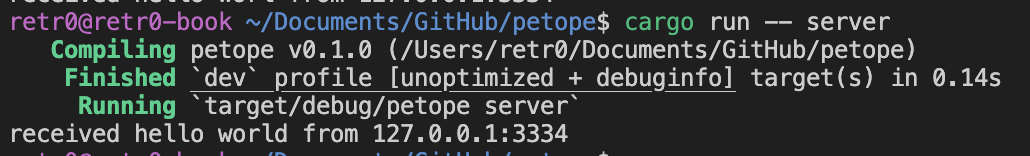
\includegraphics[width=\textwidth]{1/server.png}
  \caption{Serveri väljund, mis kuvab kliendilt vastu võetud sõnumi}
\end{figure}

\begin{figure}[H]
  \centering
  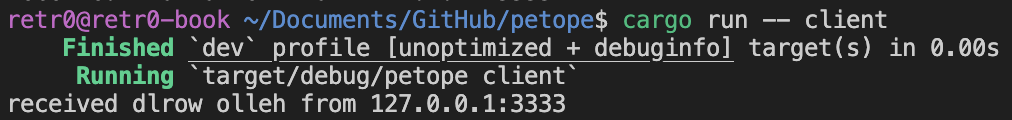
\includegraphics[width=\textwidth]{1/client.png}
  \caption{Kliendi väljund, mis kuvab serverilt saadud pööratud sõnumi}
\end{figure}

Tulemused demonstreerivad edukat suhtlust kliendi ja serveri vahel.
Klient edastas serverile sõnumi, mille järel server töötles vastuvõetud andmeid,
pöörates nende sisu ümber ning saates muudetud sõnumi kliendile tagasi.

Järgmise sammuna uuritakse teenuse avastamise mehhanisme.

\section{Sõlmede avastamine}

Pärast UDP-põhise suhtluse loomist muutub vajalikuks otsese IP-aadressimise asendamine sõlmede identifikaatoritega.
Selle saavutamiseks on vajalik avastusserver, mis seob sõlmede identifikaatorid neile vastavate IP-aadressidega.

\subsection{Avastusserver}

Implementeeritud avastusserver kasutab sama UDP-põhist protokolli,
kus sõnumid on esitatud lihttekstis stringidena järgmises formaadis:
\texttt{command|arguments}.

Kui avastusserver võtab vastu käsu, saab ta ühtlasi teada saatja lähteaadressi.
Sellest tulenevalt saab server pärast käsu \texttt{register|node id} vastuvõtmist seostada sõlme identifikaatori saatja aadressiga, näiteks:
\mintinline{js}|nodes["node id"] = "source address"|
kasutades \href{https://en.wikipedia.org/wiki/Hash_table}{paisktabelit}.

\subsection{Sõlm / peer}

Iga sõlm registreerib ennast avastusserveris ning seejärel küsib
sihtsõlme identifikaatoriga seotud aadressi.
Seda protsessi teostatakse pidevalt tsüklis, võimaldades sõlmel korduvalt
ennast registreerida, sihtaadressi hankida ning edastada sõnumeid sihtsõlmele.

\subsection{Tulemus}

Lähtekoodi käesolevas dokumendis ei esitata.
Küll aga on avastusserveri implementatsioon leitav commit'is
\href{https://github.com/dankmolot/petope/tree/5a66b32a015f395bc614a1aedc54a87a44d8dbc1}{5a66b3}.

Praeguses etapis põhineb avastusmehhanism lihttekstisel UDP-protokollil,
mis võimaldab seda testida \href{https://en.wikipedia.org/wiki/Netcat}{netcat} terminaliutiliidi abil:

\begin{figure}[H]
  \centering
  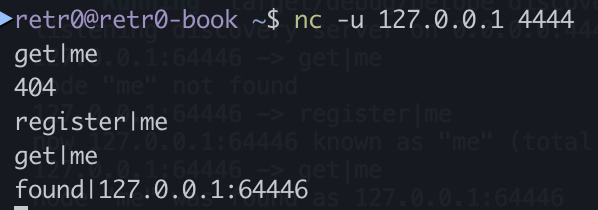
\includegraphics[width=0.7\textwidth]{2/netcat_discovery_example.png}
  \caption{Käskude saatmine netcat utiliidi abil}
\end{figure}

\begin{figure}[H]
  \centering
  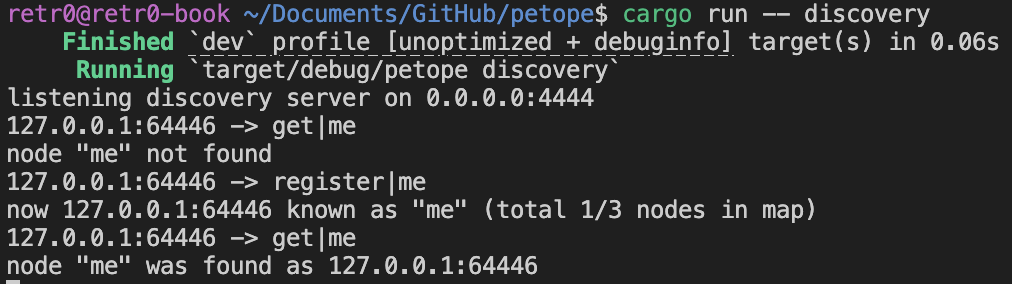
\includegraphics[width=\textwidth]{2/discovery_server_logs.png}
  \caption{Avastusserveri logiväljund}
\end{figure}

Pärast mõlema sõlme käivitamist loovad peer-id ühenduse automaatselt.

\begin{figure}[H]
  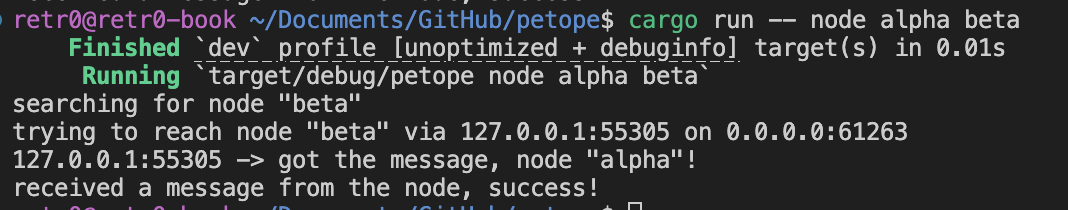
\includegraphics[width=\textwidth]{2/node_alpha.png}
  \caption{Sõlm \texttt{alpha} võtab vastu ühenduspäringu sõlmelt \texttt{beta}}
\end{figure}

\begin{figure}[H]
  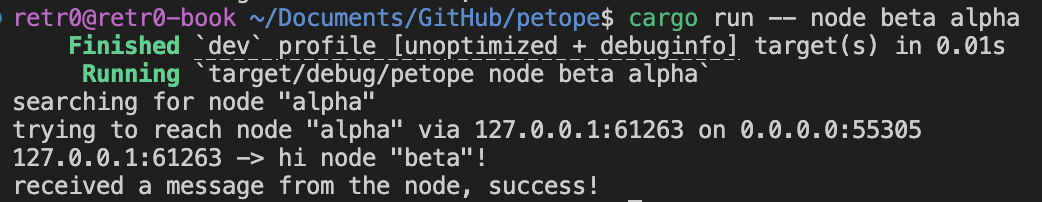
\includegraphics[width=\textwidth]{2/node_beta.png}
  \caption{Sõlm \texttt{beta} algatab ühenduse sõlmega \texttt{alpha}}
\end{figure}

Tulemused demonstreerivad, et sõlm \texttt{beta} saavutas edukalt ühenduse sõlmega \texttt{alpha},
ning sõlm \texttt{alpha} vastas sellele vastavalt.
Mõlemad sõlmed lahendasid teineteise võrguaadressid üksnes identifikaatorite
\texttt{alpha} ja \texttt{beta} abil.

Kuna praegune implementatsioon proovib pidevalt peer-sõlmi avastada ja nendega ühendust luua,
tagab see vajaliku aluse UDP hole punching'u realiseerimiseks.

\section{UDP hole punching}

UDP hole punching funktsionaalsuse hindamiseks kasutati eraldiseisvat avalikku serverit
\emph{discovery}-teenuse majutamiseks, samal ajal kui kaks sõlme paigutati erinevatesse võrkudesse.

Esimene sõlm käivitati sülearvutis, mis oli ühendatud kodusesse elamuvõrku.
Teine sõlm käivitati mobiiltelefonis, kuhu oli paigaldatud \href{https://termux.dev/en/}{Termux}
ning mis oli ühendatud Telia mobiilsidevõrku.
Discovery-server majutati renditud virtuaalses privaatserveris,
mida pakkus \href{https://www.hetzner.com/}{Hetzner} ning mis oli seadistatud staatilise avaliku IPv4-aadressiga.

\begin{figure}[H]
  \centering
  \includegraphics[width=\textwidth]{3/node_on_a_pc.png}
  \caption{Telefonist sülearvutisse saadetud edukas vastus}
  \label{fig:udp_punch_pc}
\end{figure}

\begin{figure}[H]
  \centering
  \includegraphics[width=\textwidth]{3/node_on_a_phone.png}
  \caption{Sülearvutist telefoni saadetud edukalt vastuvõetud sõnum}
  \label{fig:udp_punch_phone}
\end{figure}

Joonised \ref{fig:udp_punch_pc} ja \ref{fig:udp_punch_phone} illustreerivad edukat suhtlust
kahe sõlme vahel discovery-serveri kaudu, mis asus aadressil \emph{91.107.213.38}
\footnote{Renditud virtuaalserveri avalik IPv4-aadress}.
Sülearvuti kasutas avalikku aadressi \emph{88.196.179.131},
samal ajal kui telefon kasutas avalikku aadressi \emph{46.131.76.184}.

Mõlemad sõlmed registreerisid esmalt discovery-serveris oma avaliku lõpp-punkti informatsiooni
ning seejärel pärisid kaugema partneri lõpp-punkti informatsiooni.
Pärast seda, kui kumbki sõlm saatis teisele esialgse UDP-paketi, võimaldasid vastavad NAT-seadmed
sissetulevat liiklust, mis oli seotud loodud vastendustega. Selle tulemusel sai telefon edukalt vastu võtta sõnumi
sülearvutilt, mille järel sai sülearvuti vastuse telefonilt.

\newpage

\subsection{Täheldatud piirangud}

Esialgsed katsed viidi läbi olukorras, kus mõlemad sõlmed olid ühendatud samasse kodusesse Wi-Fi võrku.
Nendes tingimustes ei jõudnud sissetulevad paketid sõlmede vahel edukalt kohale.
Selline käitumine on tõenäoliselt seotud ruuterispetsiifilise NAT-käsitluse või kohalike pakettide edastamise mehhanismide piirangutega.
Sellest tulenevalt on samas lokaalses võrgus töötavate sõlmede jaoks vajalikud alternatiivsed partnerite avastamise ja suhtluse mehhanismid.

Ühe võimaliku lahendusena võib kasutada \href{https://en.wikipedia.org/wiki/Zero-configuration_networking}{Zeroconf}-tehnoloogiaid,
mis võimaldavad teenuste automaatset reklaamimist ja avastamist lokaalsetes võrkudes.
Sellised mehhanismid võimaldavad samas võrgus paiknevatel sõlmedel luua ühenduse ilma välise discovery-serverita.

Näiteks \href{https://docs.iroh.computer/connecting/local-discovery}{Iroh}-raamistik rakendab mDNS-laadset lokaalset avastamismehhanismi,
mida saab vajaduse korral aktiveerida.

Teine võimalik piirang tekib olukorras, kus mõlemad sõlmed paiknevad erinevates võrkudes,
kuid töötavad sama CGNAT-infrastruktuuri taga
\footnote{Seadmed jagavad sama avalikku IPv4-aadressi, säilitades samal ajal erinevad sisemised privaat-aadressid}.
Sellisel juhul ei suuda discovery-server määrata CGNAT-keskkonnas kasutatavaid sisemisi aadresse,
mis võib takistada edukat peer-to-peer ühenduse loomist.

\section{TCP hole punching}

\href{https://en.wikipedia.org/wiki/TCP_hole_punching}{TCP hole punching} töötab sarnaselt UDP hole punching mehhanismiga.
Põhimõtteliselt piisab sellest, kui mõlemad partnerid saadavad teineteise võrguaadressidele \texttt{SYN}-paketi,
mille järel võivad järgnevad paketid NAT-seadet edukalt läbida.

Peamine väljakutse seisneb sellise käitumise programmilises realiseerimises.
Enamik standardseid võrguteeke toetab TCP-pesasid, mis töötavad kas \emph{connect}-režiimis või \emph{listen}-režiimis,
kusjuures \emph{connect}-režiim võimaldab tavaliselt suhtlust ainult ühe kaugema lõpp-punktiga.

Rusti teek \href{https://crates.io/crates/socket2}{socket2} võimaldab ligipääsu operatsioonisüsteemispetsiifilistele API-dele,
mis võimaldavad TCP-pesasid taaskasutada mitme sihtaadressi jaoks, säilitades sama lokaalse pordi konfiguratsiooni.
Seda funktsionaalsust saab kasutada TCP hole punching käitumise eksperimentaalseks hindamiseks.

\subsection{Sama pesa taaskasutamine}

Katse luua mitu sama lokaalse aadressiga seotud \href{https://en.wikipedia.org/wiki/Network_socket}{pesa}
lõppeb tavaliselt veaga ``Address already in use''.
Kaasaegsed operatsioonisüsteemid pakuvad üldjuhul \texttt{SO\_REUSEPORT} pesaoptsiooni,
mis võimaldab mitmel pesal jagada sama lokaalse aadressi ja pordi kombinatsiooni.

Selle mehhanismi abil võib sõlm esmalt luua ühenduse discovery-serveriga,
et operatsioonisüsteem määraks talle lokaalse aadressi.
Seejärel võivad täiendavad pesad kasutada sama lokaalset aadressi ja porti peer-to-peer ühenduste loomisel.

Allpool on toodud näidisimplementatsioon, mis kasutab teeki \href{https://crates.io/crates/socket2}{socket2}:

\begin{figure}[H]
  \begin{minted}{rust}
use std::io;
use socket2::{Domain, Protocol, Socket, Type};

// Creates a TCP socket with SO_REUSEPORT
fn create_socket() -> io::Result<Socket> {
    let socket = Socket::new(Domain::IPV4, Type::STREAM, Protocol::TCP.into())?;
    socket.set_reuse_port(true)?; // sets SO_REUSEPORT for the socket
    Ok(socket)
}

fn main() {
    // First connect to a discovery server, so OS will give us a local addr
    let first_socket = create_socket().unwrap();
    let addr = "127.0.0.1:4444".parse().into(); // <-- discovery server
    first_socket.connect(&addr.into()).unwrap(); // establish a connection with discovery server

    let local_addr = first_socket.local_addr().unwrap()
    println!("local addr: {}", local_addr); // will print out 127.0.0.1:<random port>

    let second_socket = create_socket().unwrap();
    second_socket.bind(local_addr).unwrap(); // reuse same ip:port as in first socket
    second_socket.listen(128).unwrap(); // run socket in listen mode
}
  \end{minted}
  \caption{Näide teegi \texttt{socket2} kasutamisest taaskasutatavate pesade loomiseks}
\end{figure}

Ilma väljakutseta \mintinline{rust}|Socket::set_reuse_port(true)| lõpeb näide veaga ``Address already in use''.
Sellist käitumist on võimalik reprodutseerida, asendades väärtuse \texttt{true} väärtusega \texttt{false}.

\subsection{Esimene katse}

Discovery-serveri implementatsiooni üleviimine UDP-lt TCP-le nõudis suhteliselt väikeseid muudatusi.
Eelkõige lisati iga sissetuleva ühenduse jaoks eraldi lõim,
et vältida pesa enneaegset sulgemist.

Partner-sõlme implementatsioon osutus täiendavalt keerukaks.
Erinevalt UDP-suhtlusest nõuab TCP enne andmete edastamist loodud ühendust.
Sellest tulenevalt peab sõlm kas algatama ühenduse teise partneriga
või minema \emph{listen}-olekusse, oodates sissetulevaid ühendusi.

Esialgne implementatsioon, mis vastab commit'ile \href{https://github.com/dankmolot/petope/tree/3e83b3}{3e83b3},
töötas edukalt localhost-keskkonnas, kus mõlemad sõlmed suhtlesid \href{https://en.wikipedia.org/wiki/Loopback}{loopback}-liidese kaudu.
Kuid katsed eraldiseisvate füüsiliste seadmetega ei olnud edukad.
See tulemus viitas sellele, et ühenduse loomine ja kuulamisoperatsioonid peavad toimuma samaaegselt,
mida oli keeruline realiseerida sünkroonse Rusti koodiga.

Selle piirangu lahendamiseks võeti kasutusele asünkroonne käituskeskkond \href{https://tokio.rs/}{Tokio}.
Tokio võimaldab ühenduskatsete ja kuulamisülesannete samaaegset täitmist ühe rakenduse kontekstis.

\subsection{Teine katse}

Teine implementatsioon töötati välja \href{https://tokio.rs/tokio/tutorial}{Tokio juhendi} põhjal,
mis esitab näiteid projekti \href{https://github.com/tokio-rs/mini-redis/}{mini-redis} alusel.
Juhend pakkus struktureeritud lähenemist asünkroonse suhtluse ja protokollikäsitluse realiseerimiseks.

Rakendati lihtne \href{https://en.wikipedia.org/wiki/Frame_(networking)}{framing}-mehhanism,
mis võimaldas kasutada Rusti enumeratsioone struktureeritud sisend- ja väljundsõnumite käsitlemiseks.

Nii discovery-server kui ka sõlmede implementatsioon kirjutati ümber kasutama asünkroonseid Tokio TCP-pesasid.
Uuendatud lahenduses käivitab iga sõlm initsialiseerimise käigus taustal TCP-kuulaja,
registreerib ennast ühe korra discovery-serveris
ning proovib seejärel korduvalt luua ühendust teise sõlmega.

See implementatsioon võimaldas edukalt luua peer-to-peer TCP-suhtluse erinevate võrkude vahel.
Eksperimentaalne seadistus koosnes ühest kodusesse Wi-Fi võrku ühendatud sülearvutil töötavast sõlmest
ja teisest mobiilsidevõrgu kaudu ühendatud mobiiliseadmes töötavast sõlmest.

\begin{figure}[H]
  \centering
  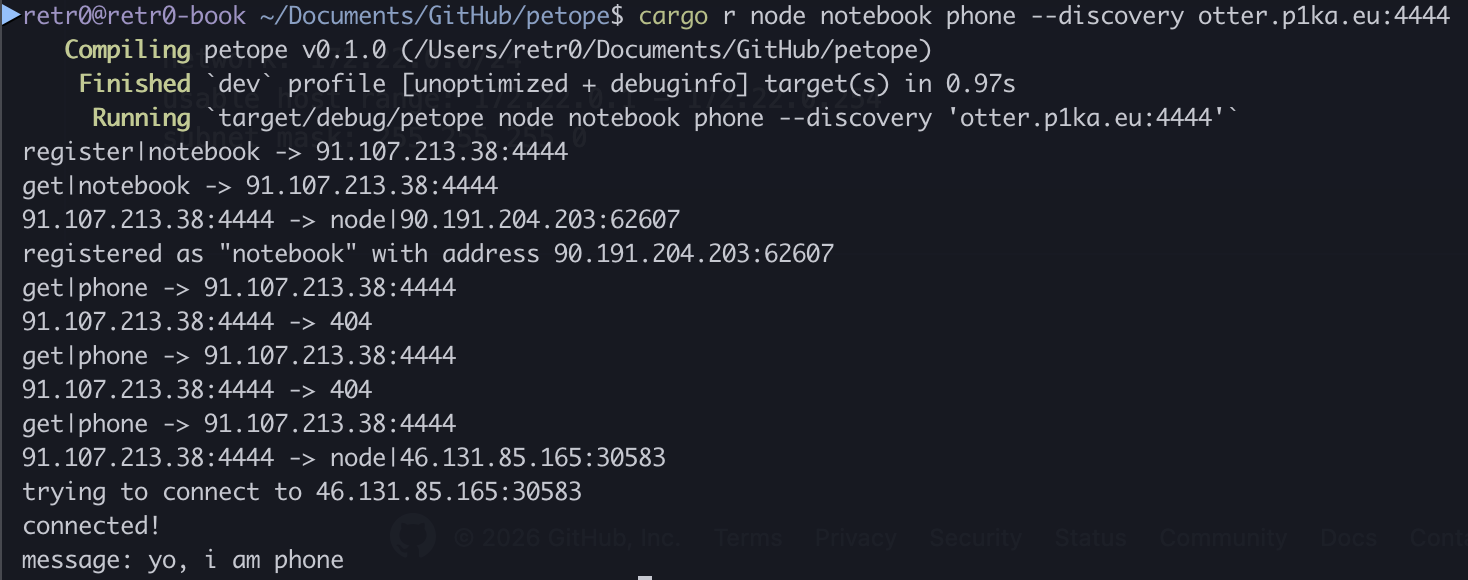
\includegraphics[width=\textwidth]{4/node_notebook.png}
  \caption{Sülearvuti sõlm otsimas ja edukalt ühendumas mobiilsõlmega}
  \label{fig:tcp_punch_notebook}
\end{figure}

\begin{figure}[H]
  \centering
  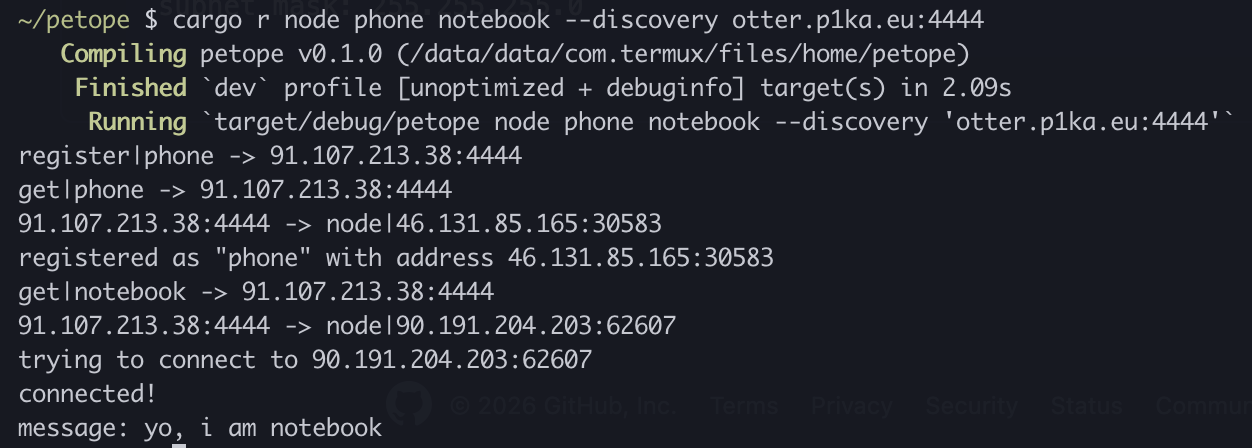
\includegraphics[width=\textwidth]{4/node_phone.png}
  \caption{Mobiilsõlm edukalt ühendumas sülearvuti sõlmega}
  \label{fig:tcp_punch_phone}
\end{figure}

Sõlmed lõid edukalt kahesuunalise ühenduse ning vahetasid identifitseerimissõnumeid kujul \texttt{"yo, i am <node name>"}.
Täheldatud käitumine viitas sellele, et ühendus loodi otse partnerite vahel, mitte TCP-kuulaja kaudu.

Samaväärset funktsionaalsust oleks tõenäoliselt olnud võimalik realiseerida üksnes Rusti standardteegi ja \emph{socket2} abil,
kuid Tokio kasutuselevõtt lihtsustas samaaegseid võrgutöid ning tõi kaasa väljakujunenud asünkroonse programmeerimise praktikad.
Selle eksperimendi implementatsioon on saadaval commit'i \href{https://github.com/dankmolot/petope/tree/c46a8e7b36c998d946180e0317b63daccaaf1a2a}{c46a8e} all.

\subsection{Sõlmed sama NAT-i taga}

Sama NAT-seadme taga paiknevad sõlmed ei suutnud endiselt luua otsest ühendust.
Selline käitumine oli ootuspärane, kuna partnerid üritasid ühenduda oma avalike IP-aadresside kaudu.
Kui avalikule IP-aadressile suunatud paketid sisenevad ruuterisse uuesti sisevõrgust,
ei pruugi ruuter olla võimeline määrama korrektset sisemist sihtkohta ning võib paketid seetõttu kõrvale jätta.

\newpage

Probleemi lahendamiseks on loodud \href{https://en.wikipedia.org/wiki/Network_address_translation#NAT_hairpinning}{NAT hairpinning} (või \emph{NAT loopback}) funktsionaalsus.
Katsetes kasutatud ruuter kuulub tootja dokumentatsiooni kohaselt seadmete hulka, mis seda funktsionaalsust toetavad,
vastavalt \href{https://www.asus.com/support/faq/1043024/}{ASUS-e dokumentatsioonile}.
Siiski ei vastanud täheldatud käitumine täielikult oodatud funktsionaalsusele.
\href{https://www.snbforums.com/threads/asus-ac86u-firmware-merlin-386-11-nat-loopback-not-working-please-help.85974/}{foorumiarutelus}
märgib kasutaja \texttt{ColinTaylor}, et NAT loopback toe toimimine võib sõltuda eksplitsiitsest pordi suunamise konfiguratsioonist,
mida käesolev implementatsioon teadlikult väldib.

See piirang motiveerib järgmises peatükis esitatud arutelu.

\section{Multiedastus-DNS}

Lisaks sõlmede avastamisele Interneti kaudu saab partnerite avastamist teostada ka
\href{https://en.wikipedia.org/wiki/Service_discovery}{teenuseavastuse} vormi abil, täpsemalt
\href{https://en.wikipedia.org/wiki/Multicast_DNS}{Multicast DNS-i (mDNS)} kaudu.
Selline lähenemine võimaldab sõlmel reklaamida oma olemasolu lokaalses võrgus, võimaldades teistel sõlmedel
see avastada ja sellega ühenduda. Selle tulemusena saavad samas lokaalses võrgus paiknevad sõlmed luua
ühendusi ilma Interneti-ühendust vajamata.

\begin{tcolorbox}
  Selline lähenemine ei võimalda suhtlust erinevates võrkudes paiknevate sõlmede vahel, mis asuvad sama
  carrier-grade NAT-i (CGNAT) taga, välja arvatud juhul, kui internetiteenuse pakkuja toetab NAT hairpinning'ut.
  IPv6 ühenduvus leevendab seda piirangut.
\end{tcolorbox}

Teenuseavastuse funktsionaalsuse realiseerimiseks kasutati
\href{https://crates.io/crates/mdns-sd}{\texttt{mdns-sd}} Rusti teeki.
Integratsioon nõudis peamiselt eelnevalt realiseeritud avastusserveri asendamist mDNS-põhise avastusega.

\subsection{Teostus}

mDNS-funktsionaalsuse integreerimine oli suhteliselt lihtne tänu teegi API lihtsusele,
mis on kontseptuaalselt sarnane eelnevalt realiseeritud avastusklientiga.
Järgmine näide demonstreerib teenuse loomist ja registreerimist
\footnote{Teenusekirje sisaldab teenuse tüüpi, IP-aadresse, hostinime, identifikaatorit ning valikulisi omadusi.}:

\begin{figure}[H]
  \begin{minted}{rust}
let sd = ServiceDaemon::new()?; // Daemon from mdns-sd
let hostname = utils::get_hostname()?; // returns current hostname with `.local.` appended
let service = ServiceInfo::new(
    "_petope._tcp.local.", // consists of a service name, protocol, and domain (.local)
    &args.id, // identificator, derived from arguments, i.e. "notebook"
    &hostname, // device hostname that must end with .local.
    (), // ip addresses, we use .enable_addr_auto() so the library will add addresses for us
    local_addr.port(), // use the same port as socket port
    None, // properties, we don't use any
)?
  // automatically populate IP addresses from network interfaces
  .enable_addr_auto();
sd.register(service)?; // ServiceDaemon will handle automatic broadcasting of the service
  \end{minted}
  \caption{Näide teenuse registreerimisest avastamiseks kasutades teeki \texttt{mdns-sd}}
\end{figure}

\newpage

Teenuseavastus on realiseeritud järgmiselt:

\begin{figure}[H]
  \begin{minted}{rust}
// fullname consists in form of identification + service type
let node_fullname = format!("{}.{}", node_id, "_petope._tcp.local.");
let receiver = sd.browse("_petope._tcp.local.")?;

loop {
    // ServiceDaemon will automatically search and resolve services for us
    let event = receiver.recv_async().await?;
    match event {
        // we just need to listen for resolved events
        ServiceEvent::ServiceResolved(svc) => {
            // Make sure that service has right identification
            if svc.get_fullname() == node_fullname.as_str() {
                let addresses = svc.get_addresses_v4();
                println!("discovered {} with addresses {:?}", node_id, addresses);
                sd.stop_browse("_petope._tcp.local.")?;

                // create SocketAddr that consists from first ipv4 address + service port
                return Ok(SocketAddr::V4(SocketAddrV4::new(
                    addresses.iter().next().unwrap().to_owned(),
                    svc.get_port(),
                )));
            }
        }
        // ignore all other events
        _ => {}
    };
}
  \end{minted}
  \caption{Partnerteenuste avastamine ja partneri IP-aadresside hankimine kasutades teeki \texttt{mdns-sd}}
\end{figure}

Ülaltoodud funktsioon blokeerib täitmise kuni sihtsõlme avastamiseni, mille järel tagastatakse vastav
võrguaadress, mida kasutatakse seejärel ühenduse loomiseks. Üheks oluliseks piiranguks on asjaolu, et
teenusetüübi vormingus oleva teenusenime komponent
(\textbf{\_name}.\_protocol.domain) ei tohi ületada 15 märki.

Eksperimentaalne hindamine näitas, et sõlmede avastamine toimub väikese latentsusega, tavaliselt lokaalses võrgus sekundi murdosa jooksul.
Täielik teostus on saadaval commit'is
\href{https://github.com/dankmolot/petope/tree/0915f06ad2b44db91ace9968bc6654252927c25b}{0915f0}.

\section{Lõpliku rakenduse arendamine}

Pärast mitme lähenemisviisi katsetamist kahe partneri vahelise peer-to-peer ühenduse loomiseks realiseeriti minimaalselt elujõuline toode (MVP), kasutades
\href{https://en.wikipedia.org/wiki/Minimum_viable_product}{iroh}
teeki. Tulemuseks olev rakendus kavandati piisavalt praktiliseks kasutamiseks isiklikes serverites ning eksperimenteerimiseks väikestes võrgukeskkondades.

Rakendus koosneb järgmistest komponentidest:
\begin{enumerate}
  \item Konfiguratsioon (Section~\ref{sec:appconfig}) --- vastutab partneri identiteedi jaoks kasutatava privaatvõtme säilitamise ning partneriteabe talletamise eest
  \item TUN-seade (Section~\ref{sec:apptun}) --- vastutab IP-pakettide vastuvõtmise ja edastamise eest hostisüsteemist
  \item Ruuter (Section~\ref{sec:approuter}) --- vastutab pakettide edastamise eest sobivale partnerile vastavalt siht-IP-aadressile
  \item Partnerid (Section~\ref{sec:apppeers}) --- ühendatud \texttt{iroh} teegi kaudu marsruuditavate IP-pakettide vahetamiseks
\end{enumerate}

Rakenduse teostus eelnes käesoleva peatüki kirjutamisele. Vastav lähtekood on saadaval commit'is
\href{https://github.com/dankmolot/petope/tree/161ffc0ae3fbb76fd88bc4d2ecf82507cd16596b}{161ffc}.

Joonis~\ref{fig:network_pipeline} illustreerib rakenduses realiseeritud pakettide marsruutimise töövoogu.

\begin{figure}[H]
  \centering
  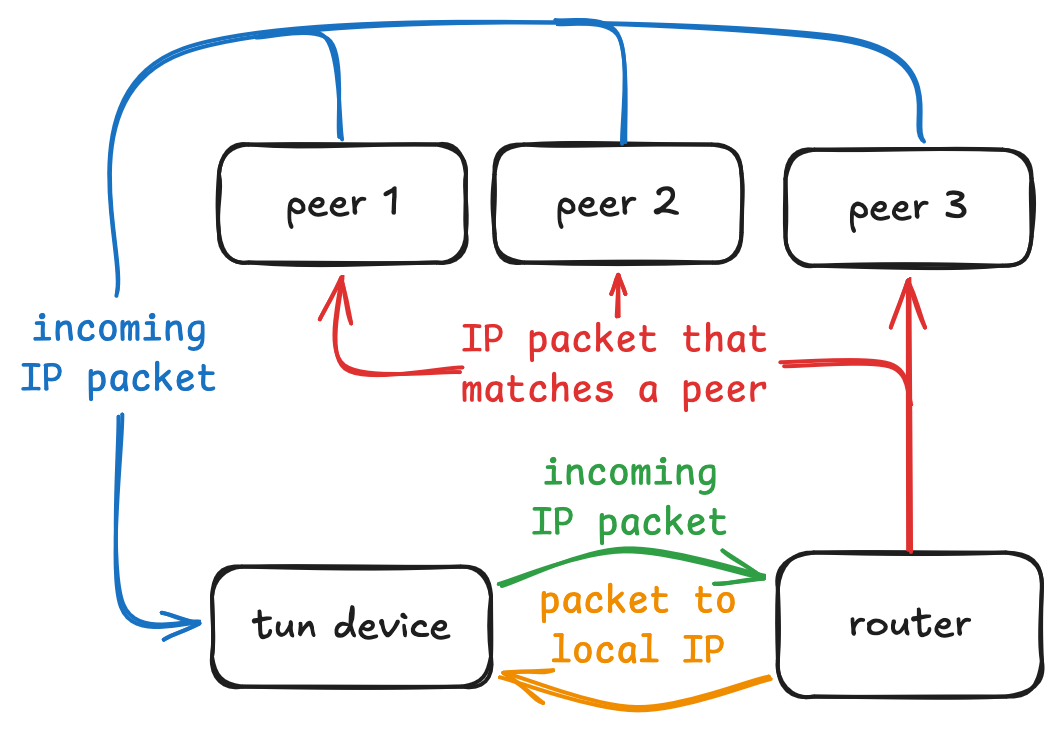
\includegraphics[width=\textwidth]{5/network_pipeline.png}
  \caption{IP-pakettide marsruutimist süsteemide vahel illustreeriv töövoog}
  \label{fig:network_pipeline}
\end{figure}

\newpage

\subsection{Konfiguratsioon} \label{sec:appconfig}

\href{https://en.wikipedia.org/wiki/Public-key_cryptography}{Krüptograafiline võtmepaar}
toimib lisaks turvamehhanismile ka sõlme identiteedina.
Avalikku võtit kasutatakse nii sõlmede avastamiseks kui ka ühenduste loomiseks.
Sellest tulenevalt tuleb privaatvõti püsivalt salvestada, et rakendus säilitaks käivituste vahel stabiilse identifikaatori ning suudaks usaldusväärselt ühenduda varem tuntud sõlmedega.

Lihtsuse huvides salvestatakse nii privaatvõti kui ka sõlmede identifikaatorid ühte konfiguratsioonifaili.
\footnote{Alternatiivse lahendusena võiks privaatvõtme eraldada eraldi faili.}
Kui konfiguratsioonis privaatvõti puudub, genereerib rakendus selle automaatselt ning salvestab konfiguratsioonifaili.

Kuna konfiguratsioon peab toetama nii lugemist kui ka muutmist olemasolevaid kommentaare ja vormingut säilitades, valiti vorminguks
\href{https://toml.io/en/}{TOML}
koos Rusti teegiga
\href{https://crates.io/crates/toml_edit}{\texttt{toml\_edit}},
mis säilitab muutmise käigus dokumendi algse struktuuri.

Kohaliku testimise hõlbustamiseks võimaldab rakendus määrata konfiguratsioonifaili asukoha käsurea argumentide kaudu.
See funktsionaalsus on realiseeritud teegi \texttt{clap} abil.

\begin{figure}[H]
  \begin{minted}{rust}
use clap::Parser;

#[derive(Parser, Debug)]
#[command(version, about, long_about = None)]
struct Cli {
    /// Path to a config file
    #[arg(short, long, default_value_t = String::from("config.toml"))]
    config: String,
}

fn main() {
    let cli = Cli::parse();
}
  \end{minted}
  \caption{Argumentide parsimine konfiguratsioonifaili valimiseks}
\end{figure}

Selline teostus võimaldab kasutada argumente \texttt{-c} või \texttt{--config}, näiteks \texttt{-c config2.toml},
alternatiivse konfiguratsioonifaili laadimiseks. Vaikimisi laadib rakendus faili \texttt{config.toml}.
Lisaks pakub teek \texttt{clap} automaatselt genereeritud abisõnumeid ja veakäsitlust.

\newpage

Järgmine funktsioon parsib konfiguratsioonifailist
\href{https://en.wikipedia.org/wiki/Base64}{Base64}-kodeeritud privaatvõtme
või genereerib uue võtme kasutades funktsiooni
\href{https://docs.rs/iroh/latest/iroh/struct.SecretKey.html#method.generate}{\texttt{SecretKey::generate()}}.
Kui genereeritakse uus võti, kirjutatakse uuendatud konfiguratsioon tagasi kettale.

\begin{figure}[H]
  \begin{minted}{rust}
fn get_or_generate_secret_key(path: &str, doc: &mut DocumentMut) -> Result<SecretKey> {
    // get a global "private_key" value from parsed file
    if let Some(encoded) = doc.get("private_key").and_then(|v| v.as_str()) {
        // try to parse string from base64 into bytes
        let decoded =
            utils::base64_decode(encoded).context("private key must be encoded in base64")?;

        // convert to &[u8] and use TryInto which is implemented in SecretKey
        decoded
            .as_slice()
            .try_into()
            .context("private key must be valid ed25519 key bytes encoded in base64")
    } else {
        // No value, no problem, just generate a new
        let key = SecretKey::generate();

        // insert base64 encoded bytes of private key into document
        doc.insert(
            "private_key",
            utils::base64_encode(&key.clone().to_bytes()).into(),
        );

        // and write back to the original file
        std::fs::write(path, doc.to_string())
            .with_context(|| format!("write {} with generated private key", path))?;

        Ok(key)
    }
}
  \end{minted}
  \caption{Funktsioon privaatvõtme parsimiseks või genereerimiseks}
\end{figure}

\newpage

Kuna privaatvõtit on vaja ainult lõpp-punkti loomise ajal,
\footnote{Privaatvõtit kasutatakse üksnes lõpp-punkti initsialiseerimisel ning seda ei ole pärast seda vaja säilitada.}
parsitatakse ülejäänud konfiguratsiooniandmed, näiteks sõlmede definitsioonid, sellest sõltumatult.

\begin{figure}[H]
  \begin{minted}{rust}
use iroh::{EndpointId, SecretKey};
use toml_edit::{DocumentMut, Item, Table};

#[derive(Debug, Clone)]
pub struct Config {
    pub peers: Vec<Peer>,
}

#[derive(Debug, Clone)]
pub struct Peer {
    pub id: EndpointId,
}

impl Config {
    fn parse(doc: DocumentMut) -> Result<Self> {
        // iterate over array of tables which looks like this in toml
        // [[peer]]
        // ...
        //
        // [[peer]]
        // ...
        let mut peers = Vec::new();
        if let Some(arr) = doc.get("peer").and_then(Item::as_array_of_tables) {
            for (i, t) in arr.iter().enumerate() {
                peers.push(
                    // here is parsing of each individual peers happens
                    Peer::parse(t).with_context(|| format!("parse a [[peer]] at index {}", i))?,
                );
            }
        }

        Ok(Config { peers })
    }
}

impl Peer {
    fn parse(t: &Table) -> Result<Self> {
        // gets "id" key as a string
        let id = t
            .get("id")
            .and_then(Item::as_str)
            .ok_or_else(|| anyhow!("expected an `id` but got nothing"))?;

        // Use alias to PublicKey::from_z32 to parse z32 string to public key
        let id = EndpointId::from_z32(id).context("parse `id` as an EndpointId")?;

        Ok(Peer { id })
    }
}

  \end{minted}
  \caption{Funktsioonid sõlmede konfiguratsiooni parsimiseks}
\end{figure}

\newpage

Lõpuks ühendatakse funktsioonid \texttt{Config::parse} ja \texttt{get\_or\_generate\_secret\_key} üheks laadimisfunktsiooniks,
mida kutsutakse rakenduse initsialiseerimise käigus.

\begin{figure}[H]
  \begin{minted}{rust}
impl Config {
    pub fn load(path: &str) -> Result<(SecretKey, Config)> {
        // just std::fs::read_to_string(path) which returns an empty string if file
        let data = Config::read_file(path).with_context(|| format!("read config from {}", path))?;

        // Parse into DocumentMut since we modify it in Config::get_or_generate_secret_key
        let mut doc = data
            .parse::<DocumentMut>()
            .with_context(|| format!("parse {}", path))?;

        let private_key =
            Config::get_or_generate_secret_key(path, &mut doc).context("get private key")?;

        // Return private key and config seperately
        Ok((private_key, Config::parse(doc)?))
    }
}

fn main() -> Result<()> {
    // ...
    let (secret_key, config) = Config::load(&cli.config).context("load config")?;
    // secret_key can be later used in Endpoint::builder(...).secret_key(secret_key)
}
  \end{minted}
  \caption{Konfiguratsiooni laadimise funktsioon}
\end{figure}

Selline ülesehitus võimaldab rakendusel säilitada oma privaatvõtit, hoides samal ajal kaugsõlmede avalikke identifikaatoreid.
Kuigi teostus lisab süsteemile täiendavat keerukust, säilitab see paindlikkuse konfiguratsioonisüsteemi edaspidiseks laiendamiseks.

\subsection{TUN-seade} \label{sec:apptun}
\href{https://en.wikipedia.org/wiki/TUN/TAP}{TUN-seade} on \href{https://en.wikipedia.org/wiki/Network_virtualization}{virtuaalne võrguliides},
mis võimaldab tarkvararakendustel saata ja vastu võtta \href{https://en.wikipedia.org/wiki/Internet_Protocol}{IP-pakette}. TUN-seadmeid kasutatakse tavaliselt VPN-lahendustes
\footnote{Mõned teostused kasutavad selle asemel TAP-seadmeid, mis töötavad MAC-kihis ja võimaldavad ligipääsu Etherneti kaadritele.},
ning need sobivad käesoleva projekti jaoks, kuna võimaldavad tuletada IP-aadresse võrdseadmete lõpp-punkti identifikaatoritest, võimaldades suhtlust standardse võrgutarkvara kaudu.

Valiti \href{https://crates.io/crates/tun-rs/}{\texttt{tun-rs}} teek, kuna see toetab kõiki peamisi lauaarvutite operatsioonisüsteeme.

\newpage

TUN-seadme initsialiseerimiseks pakub \texttt{tun-rs} kompaktset konfiguratsiooniliidest:
\begin{figure}[H]
  \begin{minted}{rust}
use tun_rs::{AsyncDevice, DeviceBuilder};

fn create_device() -> std::io::Result<AsyncDevice> {
    DeviceBuilder::new()
        .name("petope0") // seadme nimi, mida kuvatakse ifconfig käsus
        .mtu(65535) // MTU, tavaliselt 1500, Linuxis ipv6 jaoks minimaalne 1280
        .ipv4("10.0.0.1", 32, None)
        .ipv6("fdaa::beaf", 128)
        .layer(tun_rs::Layer::L3) // määra TUN-seadme jaoks L3, TAP jaoks L2
        .build_async()
}
  \end{minted}
  \caption{Näide TUN-seadme loomisest \texttt{tun-rs} teegi abil}
  \label{code:create_tun}
\end{figure}

IP-pakettide saatmiseks ja vastuvõtmiseks pakub teek kõrgema taseme abstraktsiooni
\href{https://docs.rs/tun-rs/2.8.3/tun_rs/struct.AsyncDevice.html}{AsyncDevice}
üle \href{https://docs.rs/tun-rs/2.8.3/tun_rs/async_framed/index.html}{async\_framed}
mooduli kaudu. See abstraktsioon võimaldab kasutada asünkroonset liidest pakettide töötlemiseks, vältides vajadust töötada käsitsi toor-baidivoogudega.
\begin{figure}[H]
  \begin{minted}{rust}
use tun_rs::async_framed::DeviceFramed;
use futures::{SinkExt, StreamExt};

// oluline on ümbritseda AsyncDevice Arc-iga,
// et seda oleks võimalik jagada
let dev = Arc::new(create_device().unwrap());
// loo DeviceFramed ja jaga saatmise ja vastuvõtu osadeks
let (mut rx, mut tx) = DeviceFramed::new(dev, BytesCodec::new()).split();

// ülesanne, mis võtab vastu IP-pakette
tokio::spawn(async move {
    // kasuta vastuvõtuks futures::StreamExt liidest
    while let Some(frame) = rx.next().await {
        match frame {
            Ok(bytes) => {
                // töötle sissetulevat IP-paketti "bytes" muutujast
            }
            Err(e) => eprintln!("raami parsimine tun-seadmest: {:?}", e),
        }
    }
});

// ülesanne, mis saadab pakette
tokio::spawn(async move {
    // võta pakett mingist kanalist
    if let Err(e) = tx.send(bytes).await {
        eprintln!("baitide teisendamine raamiks tun-seadmesse: {:?}", e);
    }
});
  \end{minted}
  \caption{Näide asünkroonsest pakettide saatmisest ja vastuvõtmisest \texttt{tun-rs} abil}
\end{figure}

Teostus integreerub otseselt Tokio pakutava asünkroonse täitmismudeliga, lihtsustades samaaegset pakettide töötlemist.

\newpage

\subsubsection{Suure MTU kohta} \label{sec:hugemtu}
Nagu näidatud loendis~\ref{code:create_tun}, on TUN-seade konfigureeritud MTU väärtusega 65535.

See konfiguratsioon põhineb
\href{https://yggdrasil-network.github.io/2018/07/13/about-mtu.html}{Yggdrasili blogipostituses}
esitatud arutelul suurte MTU väärtuste ja \href{https://en.wikipedia.org/wiki/Path_MTU_Discovery}{Path MTU Discovery} kohta.
Path MTU Discovery võimaldab vahepealsetel süsteemidel teavitada lõpp-punkte olukorrast, kus paketid ületavad toetatud edastussuuruse, võimaldades fragmenteerimist sobiva MTU väärtuse juures.

Suurem MTU võib süsteemi tulevastes iteratsioonides vähendada fragmenteerimise üldkulu, vähendades potentsiaalselt nii ribalaiuse üldkulu kui ka paketifragmentatsiooniga seotud protsessorikasutust.

\subsubsection{Täiendavate marsruutide lisamine}
Selles etapis sisaldab TUN-seade ainult lokaalselt määratud IP-aadresse. Operatsioonisüsteemi marsruutimistabel peab siiski sisaldama ka võrdseadmete aadresside marsruute
(vt jaotis~\ref{sec:apppeers}), et võrdseadmetele suunatud paketid edastataks läbi TUN-liidese.

Marsruutimistabeli kirjete haldamiseks kasutati \href{https://crates.io/crates/net-route}{\texttt{net-route}} teeki, kuna see toetab platvormiülest marsruutide haldust.
Järgmine näide demonstreerib, kuidas lisada TUN-seadmega seotud IPv4 marsruuti:
\begin{figure}[H]
  \begin{minted}{rust}
use net_route::{Handle, Route};

// handle kasutatakse süsteemi marsruutimistabeli haldamiseks
let handle = net_route::Handle::new().unwrap();
// liidese indeksit kasutatakse marsruutide seostamiseks TUN-seadmega
let ifindex = dev.if_index().unwrap();

// IP-aadress ja prefiks
let route = Route::new("10.0.0.2".parse().unwrap(), 32)
    .with_ifindex(ifindex);

handle.add(&route).await.unwrap(); // lisa ülaltoodud marsruut marsruutimistabelisse
  \end{minted}
  \caption{Näide marsruudi lisamisest \texttt{net-route} teegi abil}
\end{figure}

Pärast marsruudi lisamist edastatakse määratud sihtkohta adresseeritud paketid läbi TUN-liidese,
võimaldades rakendusel neid töödelda.

\newpage

\subsection{Marsruuter} \label{sec:approuter}

Marsruuteri komponent vastutab IP-pakettide saatmise ja vastuvõtmise eest.
Seetõttu on vajalik tõhus mehhanism paketandmete edastamiseks asünkroonsete ülesannete vahel.

\href{https://en.wikipedia.org/wiki/Channel_(programming)}{Kanaleid} kasutatakse tavaliselt suhtluseks lõimede ja asünkroonsete ülesannete vahel.
Tokio pakub selleks \href{https://docs.rs/tokio/latest/tokio/sync/mpsc/index.html}{\texttt{tokio::sync::mpsc}}
moodulit. Standardsed järjekorrapõhised kanalid säilitavad siiski vanemad sõnumid kuni nende töötlemiseni, eelistades seeläbi varasemaid pakette uuematele.
Selline käitumine võib negatiivselt mõjutada latentsustundlikke töökoormusi, sealhulgas
\href{https://en.wikipedia.org/wiki/Real-time_communication}{reaalajas suhtlussüsteeme}.

Selle piirangu lahendamiseks valiti \href{https://github.com/brunocodutra/ring-channel}{\texttt{ring-channel}} teek.
See teek realiseerib \href{https://en.wikipedia.org/wiki/Circular_buffer}{ring-buffer}-il põhineva kanali
koos \href{https://en.wikipedia.org/wiki/Non-blocking_algorithm}{lock-free} sünkroniseerimissemantikaga.
Kui puhvri maht ületatakse, kirjutatakse vanemad paketid uuemate poolt üle, võimaldades süsteemil ülekoormuse perioodil aegunud andmed kõrvale jätta.

Kuna TUN-seadmest vastuvõetud andmed koosnevad toor-baidijadadest, kasutatakse IP-pakettide parsimiseks \href{https://crates.io/crates/etherparse}{\texttt{etherparse}}
teeki. Järgmine näide illustreerib selle kasutamist marsruuteri teostuses:
\begin{figure}[H]
  \begin{minted}{rust}
fn route(
    // TUN-seadmest saadud baidid
    bytes: Bytes,
    // TUN-seadmele suunatud ring-channel puhver
    to_network_tx: &RingSender<Bytes>
) -> Result<()> {
    // parsi baidid etherparse teegi IP-paketiks
    let ip = IpSlice::from_slice(&bytes[..]).context("sissetuleva IP-paketi parsimine")?;
    // IpAddr, kust pakett pärineb
    let src = ip.source_addr();
    // IpAddr, kuhu pakett on suunatud
    let dst = ip.destination_addr();

    // tegemist on lokaalse paketiga, tagasta see kernelile
    if src == dst {
        let _ = to_network_tx.send(bytes);
        return Ok(());
    }

    // TODO: saada paketid erinevatele võrdseadmetele IP-aadressi alusel
    
    Ok(())
}
  \end{minted}
  \caption{Marsruutimisfunktsioon, mis parsib toorbaitidest IP-paketid aadressipõhiseks marsruutimiseks}
\end{figure}

See teostus võimaldab juba lokaalset paketitöötlust läbi TUN-liidese ilma keeruka marsruutimisloogika vajaduseta.
Olemasolev Rusti ökosüsteem vähendab märkimisväärselt teostuse keerukust, pakkudes korduvkasutatavaid abstraktsioone IP-pakettide parsimiseks ja asünkroonseteks võrgutoiminguteks.

\subsection{Sõlmed} \label{sec:apppeers}

Rakenduse sõlmede komponent vastutab ühenduste haldamise ja andmete edastamise eest.
Ruuteri komponent suunab TUN-seadmest vastuvõetud paketid sihtaadressi alusel vastavale sõlmele.

\subsubsection{Sõlme identifikaatorite teisendamine IP-aadressideks}

Aadresside määramise lähenemine on inspireeritud Yggdrasil-i disainist, kus IPv6-aadressid tuletatakse sõlmede avalikest võtmetest.
Sarnane mehhanism on realiseeritud ka käesolevas projektis.
\begin{figure}[H]
  \begin{minted}{rust}
// converts EndpointId into an ipv4 address in 10.0.0.0/8 subnet
fn ipv4_from_id(id: &EndpointId) -> Ipv4Addr {
    Ipv4Addr::new(10, id[0], id[1], id[2])
}

// joins two u8 integers into one u16 integer
fn u8_pair(a: u8, b: u8) -> u16 {
    ((a as u16) << 8) | b as u16
}

// converts EndpointId into an ipv6 address in fd22::/16 subnet
fn ipv6_from_id(id: &EndpointId) -> Ipv6Addr {
    Ipv6Addr::new(
        0xfd22,
        u8_pair(id[0], id[1]),
        u8_pair(id[2], id[3]),
        u8_pair(id[4], id[5]),
        u8_pair(id[6], id[7]),
        u8_pair(id[8], id[9]),
        u8_pair(id[10], id[11]),
        u8_pair(id[12], id[13]),
    )
}
  \end{minted}
  \caption{\texttt{EndpointId} väärtuste teisendamine IP-aadressideks}
\end{figure}

Need funktsioonid võimaldavad rakendusel genereerida deterministlikke IP-aadresse nii \emph{TUN-liidesele} kui ka ühendatud \emph{sõlmedele}.
Kuna aadressid tuletatakse otseselt avalikust võtmest, saavad mõlemad suhtlusosapooled sõltumatult identsed aadressimäärangud.

\newpage

\subsubsection{Paketide marsruutimine sõlmedele}

Paketide marsruutimist ruuterist individuaalsetele sõlmedele saab seejärel realiseerida sihtkoha IP-aadresside abil:
\begin{figure}[H]
  \begin{minted}{rust}
// example of peer structure
struct Peer {
    pub id: EndpointId,
    pub ipv4: Ipv4Addr,
    pub ipv6: Ipv6Addr,
}

impl Peer {
  pub fn new(id: EndpointId) -> Self {
    Peer {
        id,
        ipv4: ipv4_from_id(id),
        ipv6: ipv6_from_id(id),
    }
  }

  pub async fn send(&self, bytes: Bytes) {
    // TODO: connect to the peer and send packet
  }
}

// map of IpAddr to a Peer for routing packets from TUN device
let routes: HashMap<IpAddr, Arc<Peer>> = HashMap::new();
// Example peer
let peer = Arc::new(Peer::new("abcdef...")); // wrapped around Arc<...> so it can be shared

// Add both ipv4 and ipv6 addresses to point to the peer
routes.insert(IpAddr::V4(peer.ipv4), peer.clone());
routes.insert(IpAddr::V6(peer.ipv6), peer.clone());

// Router route function from Router section
fn route(
    bytes: Bytes,
    // ...
) {
    // ip packet parsed here with dst IpAddr
    // ...

    if let Some(target) = routes.get(&dst) {
        target.send().await;
        return;
    }
}
  \end{minted}
  \caption{IP-põhine marsruutimine individuaalsetele sõlmedele}
\end{figure}

\newpage

\subsubsection{Ühenduse loomine sõlmega}

Enne pakettide edastamist tuleb esmalt luua ühendus sõlmede vahel.
Andmeid saata sooviv sõlm algatab ühenduse, samal ajal kui kaugpoolne sõlm aktsepteerib sissetulevaid ühendusi.
Ühenduse loomise saab realiseerida järgnevalt:
\begin{figure}[H]
  \begin{minted}{rust}
// presets::N0 contain n0 provided relays and discovery services
let endpoint = Endpoint::builder(presets::N0)
    .secret_key(secret_key) // secret key retrived from config previouly
    .alpns(vec![b"petope/0"]) // special string which indicates what protocols are supported
    .bind() // builds Endpoint
    .await
    .unwrap();

// try to connect to the peer by id
let conn = endpoint.connect(peer.id, b"petope/0").await.unwrap()

// here connection can be cached and used to send and receive data
  \end{minted}
  \caption{Ühenduse algatamine sõlmega}
\end{figure}

Sissetulevate ühenduste vastuvõtmine nõuab täiendavat käsitlemist:
\begin{figure}[H]
  \begin{minted}{rust}
// additional map to get a peer by its id
let peers: HashMap<EndpointId, Arc<Peer>> = HashMap::new();

// store example peer from previous code
peers.insert(peer.id, peer);

// receive incoming connections until Endpoint was stopped
while let Some(incoming) = endpoint.accept().await {
    // finish handshake and get a connection
    let conn = incoming.await.unwrap() 
    // find related peer and store connection in it
    if let Some(peer) = peers.get(&conn.remote_id()) {
        // TODO: cache connection in peer
    }
}
  \end{minted}
  \caption{Sissetulevate ühenduste vastuvõtmine sõlmedelt}
\end{figure}

Eelnevates näidetes on ühenduste vahemällu salvestamise implementatsioon välja jäetud.
Kuna rakendus on asünkroonne, võivad mitmed lõimed samaaegselt pääseda ligi vahemällu salvestatud ühendustele ning neid võidakse käitusajal ka asendada.
Ühe võimaliku sünkroniseerimisprimitiivina saab kasutada
\href{https://doc.rust-lang.org/std/sync/struct.Mutex.html}{\texttt{std::sync::Mutex}},
kuigi ühendusi eeldatavasti loetakse oluliselt sagedamini kui muudetakse.
Sobivam alternatiiv on
\href{https://doc.rust-lang.org/std/sync/struct.RwLock.html}{\texttt{std::sync::RwLock}},
mis võimaldab samaaegset lugemisjuurdepääsu.
Käesolevas implementatsioonis kasutatakse siiski
\href{https://docs.rs/arc-swap/latest/arc_swap/}{\texttt{arc\_swap}} teeki,
kuna see võimaldab jagatud väärtuste efektiivset atomaarset asendamist minimaalse sünkroniseerimiskuluga.

\newpage

Järgmine funktsioon salvestab ja asendab vahemällu salvestatud ühendusi:
\begin{figure}[H]
  \begin{minted}{rust}
struct Peer {
    // ...
    // ArcSwapOption is used since connection can be uninitalized
    conn: ArcSwapOption<Connection>
}

impl Peer {
    pub fn set_connection(&self, conn: Arc<Connection>) {
        // replace old value with new connection
        if let Some(old) = self.conn.swap(Some(conn)) {
            // if there was existing connection, close it
            old.close(VarInt::from_u32(0), b"outdated");
        }
    }
}
  \end{minted}
  \caption{Taaskasutatava ühenduse salvestamise funktsioon}
\end{figure}

Ühendused hangitakse üldjuhul alles siis, kui andmete edastamine on vajalik.
Seetõttu võib ühenduse hankimise funktsioon automaatselt luua ka uue ühenduse, kui aktiivne ühendus puudub:
\begin{figure}[H]
  \begin{minted}{rust}
impl Peer {
    // get a connection without automatically connecting
    pub fn try_get_connection(&self) -> Option<Arc<Connection>> {
        self.conn
            .load_full()
            // return a connection only if it wasn't closed
            .filter(|conn| conn.close_reason().is_none())
    }

    // gets current non-closed connection or tries to make a connection
    pub async fn get_connection(&self) -> Result<Arc<Connection>, ConnectError> {
        // try to get an existing connection
        if let Some(conn) = self.try_get_connection() {
            return Ok(conn);
        }

        // or try to connect
        match self.endpoint.connect(self.id, ALPN).await {
            Ok(conn) => {
                // connection must be wrapped in Arc due to ArcSwap
                let conn = Arc::new(conn);
                // store connection so it will be reused later
                self.set_connection(conn.clone());
                Ok(conn)
            }
            // just return an error if was unsuccessful
            Err(e) => Err(e),
        }
    }
}
  \end{minted}
  \caption{Funktsioon olemasoleva ühenduse hankimiseks või uue ühenduse loomiseks}
\end{figure}

\newpage

\subsubsection{Pakettide fragmenteerimise taotlemine}

Ülejäänud funktsionaalsus hõlmab IP-pakettide saatmist ja vastuvõtmist sõlmede vahel.
Nagu kirjeldatud jaotises~\ref{sec:hugemtu}, on TUN-seadme MTU väärtuseks määratud \emph{65535}, mis ületab tavapärase Etherneti MTU suuruse ligikaudu 1500 baiti.
Sellest tulenevalt on vajalik kasutada Path MTU Discovery mehhanismi, et tagada pakettide korrektne fragmenteerimine.

\texttt{iroh} ühendusliides pakub minimaalset toetatud MTU väärtust, mida saab kasutada ICMP-vastuste genereerimiseks, et teavitada operatsioonisüsteemi paketi suuruse vähendamise vajadusest.
Kuigi ICMP seostatakse sageli utiliitidega nagu \texttt{ping}, mängib see olulist rolli ka võrguvigade raporteerimisel ja Path MTU Discovery protsessis.
Kogu ICMP liikluse blokeerimine võib negatiivselt mõjutada võrgu toimimist ning seda tuleks üldjuhul vältida.
Selle asemel tuleks vajadusel filtreerida üksnes spetsiifilisi sõnumitüüpe.

Vastavalt
\href{https://datatracker.ietf.org/doc/html/rfc4443#section-3.2}{RFC 4443}-le
defineerib ICMPv6 \emph{Packet Too Big} sõnumi (tüüp 2, kood 0), mis teavitab saatjat, et edastatud pakett ületab toetatud MTU suuruse.
Vastus peab sisaldama ka osa algsest IP-paketist.
\begin{figure}[H]
  \begin{minted}{rust}
// returns an icmp response that fragmentation is needed, payload must be the same as ip slice
pub fn fragmentation_needed_response(ip: &IpSlice, payload: &[u8], mtu: usize) -> BytesMut {
    match ip {
        IpSlice::Ipv4(v4) => {} // very similar to ipv6 version
        IpSlice::Ipv6(v6) => {
            let header = v6.header();
            // convert given mtu in u32, or use maximum u32 integer
            let mtu = mtu.try_into().unwrap_or(std::u32::MAX);
            // create a packet destined back to source with PacketTooBig message
            let builder = PacketBuilder::ipv6(header.destination(), header.source(), HOP_LIMIT)
                .icmpv6(Icmpv6Type::PacketTooBig { mtu });

            // cut original IP packet so it will fit into MTU
            let payload_len = payload.len().min(mtu as usize - header.slice().len());
            let payload = &payload[..payload_len];

            // write icmp packet into a buffer and return it
            let mut writer = BytesMut::with_capacity(builder.size(payload.len())).writer();
            builder.write(&mut writer, payload).unwrap();
            writer.into_inner()
        }
    }
}
  \end{minted}
  \caption{ICMP \emph{Packet Too Big} vastuse loomise funktsioon}
\end{figure}

\newpage

\subsubsection{Pakettide saatmine sõlmedele}

Järgnev implementatsioon ühendab eelnevalt kirjeldatud funktsionaalsuse terviklikuks pakettide edastamise mehhanismiks:
\begin{figure}[H]
  \begin{minted}{rust}
impl Peer {
    fn send(&self, bytes: Bytes) -> Result<(), SendDatagramError> {
        match self.get_connection() {
            Ok(conn) => {
                // check first if packet fits into MTU
                if let Some(max) = conn.max_datagram_size() {
                    // if not, notify sender to reduce packet size
                    if bytes.len() > max {
                        self.handle_too_big(bytes, max);
                        return Ok(());
                    }
                }

                // simply send bytes to the connection
                conn.send_datagram(bytes)
            }
            Err(e) => {
              eprintln!("unable to connect to {}: {:?}", self.id, e);
              Ok(())
            }
        }
    }

    fn handle_too_big(&self, bytes: Bytes, mtu: usize) {
        // parse bytes into an ip slice
        let ip = IpSlice::from_slice(&bytes[..]).unwrap();
        // create an icmp response based on original packet
        let response = fragmentation_needed_response(&ip, &bytes[..], mtu);
        // send response to the TUN interface
        let _ = self.to_network_tx.send(response.freeze());
    }
}
  \end{minted}
  \caption{Täielik pakettide edastamise funktsioon sõlme jaoks}
\end{figure}

Datagrammide vastuvõtmine on võrreldes eelnevaga märksa lihtsam ning seisneb peamiselt funktsiooni 
\texttt{conn.read\_datagram()} korduvates väljakutsetes ja vastuvõetud pakettide edastamises TUN-seadmele kasutades
\texttt{to\_network\_tx.send(bytes)}.

Integreerides eelnevalt kirjeldatud komponendid, sealhulgas konfiguratsiooni halduse, marsruutimise, 
sõlmedevahelise suhtluse ja pakettide käsitlemise, võimaldab lõplik implementatsioon toimivat peer-to-peer VPN-lahendust, 
milles sõlmed konfigureeritakse lokaalselt.

\section{Rakenduse testimine ja hindamine}

Kuna rakendus on implementeeritud Rust programmeerimiskeeles, tuleb see enne käivitamist kompileerida.
Ametlik \href{https://rust-lang.org/learn/get-started/}{Get Started leht} sisaldab paigaldusjuhiseid
\href{https://en.wikipedia.org/wiki/Software_development_kit}{Rust SDK} jaoks toetatud süsteemidel.

Rakenduse saab kompileerida käsu \texttt{cargo build} käivitamisega. Tulemuseks olev käivitatav fail genereeritakse
asukohas \texttt{target/debug/petope}, mida saab seejärel käivitada käsurealiidesest. Kuna rakendus loob
ja kasutab TUN-seadet, on vajalikud administraatoriõigused. Linuxi süsteemides tuleks käivitatav fail seetõttu
käivitada kasutades \texttt{sudo}, näiteks:
\texttt{sudo ./target/debug/petope}.

Esimesel käivitamisel genereerib rakendus konfiguratsioonifaili \texttt{config.toml} ning kuvab tööaja informatsiooni,
nagu on näidatud järgneval joonisel:
\begin{figure}[H]
  \centering
  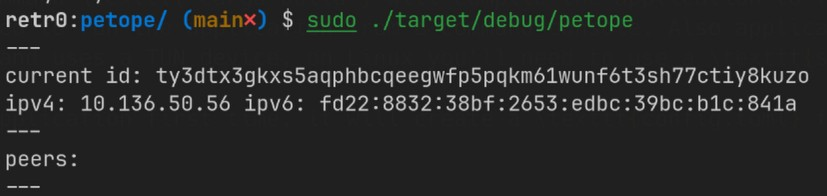
\includegraphics[width=\textwidth]{5/first_run.jpg}
  \caption{Rakenduse väljund esmakordsel käivitamisel, kuvades sõlme identifikaatori, määratud IP-aadressid ning tühja sõlmede loendi}
\end{figure}

\begin{figure}[H]
  \centering
  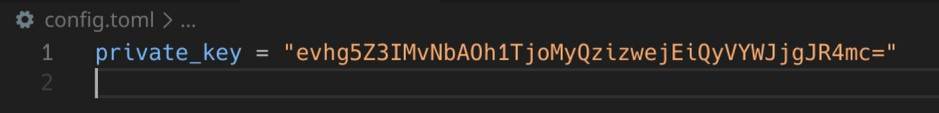
\includegraphics[width=\textwidth]{5/first_run_config.jpg}
  \caption{Genereeritud \texttt{config.toml} faili sisu pärast esmakordset käivitamist}
\end{figure}

Rakendus kuvab kohaliku sõlme identifikaatori ning määratud IP-aadressid. Genereeritud konfiguratsioonifail
sisaldab algselt ainult privaatvõtme välja, mis tagab, et sõlme identiteet jääb rakenduse taaskäivituste vahel püsivaks.

Seejärel käivitati rakendus teises arvutis, et saada selle sõlme identifikaator ja määratud aadressid:
\begin{figure}[H]
  \centering
  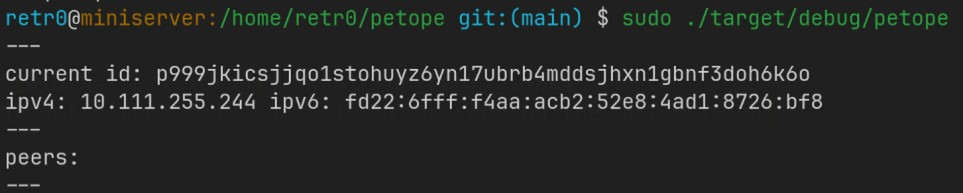
\includegraphics[width=\textwidth]{5/first_run_server.jpg}
  \caption{Rakendus töötamas teises arvutis}
\end{figure}

\newpage

Pärast mõlema sõlme identifikaatorite ja IP-aadresside saamist uuendati vastavalt sõlmede konfiguratsiooni:
\begin{figure}[H]
  \centering
  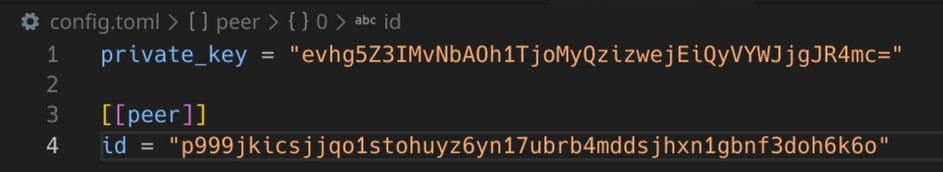
\includegraphics[width=\textwidth]{5/config_with_peer.jpg}
  \caption{Uuendatud \texttt{config.toml} fail, mis sisaldab teise arvuti sõlme konfiguratsiooni}
\end{figure}

Sama protseduuri korrati teises arvutis, kasutades esimese sõlme identifikaatorit.
Pärast rakenduse taaskäivitamist kuvati sõlmede loendis korrektselt konfigureeritud sõlm koos vastavate IP-aadressidega.
\begin{figure}[H]
  \centering
  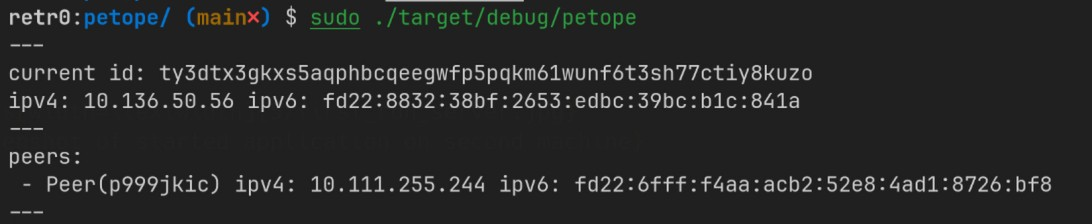
\includegraphics[width=\textwidth]{5/second_run.jpg}
  \caption{Rakenduse väljund pärast kaugsõlme konfigureerimist}
\end{figure}

Rakenduse töötamise ajal oli võimalik luua ühendus teise arvutiga, kasutades rakenduse poolt määratud IP-aadresse.
Esimese kaugsõlmele suunatud IP-paketi edastamisel lahendas rakendus sõlme identifikaatori, lõi esmase ühenduse läbi
\href{https://docs.iroh.computer/concepts/relays}{relee} ning seejärel vahendas otsese
\href{https://en.wikipedia.org/wiki/Peer-to-peer}{peer-to-peer} ühenduse. Sellist käitumist on võimalik jälgida ICMP kajapäringute saatmisel:
\begin{figure}[H]
  \centering
  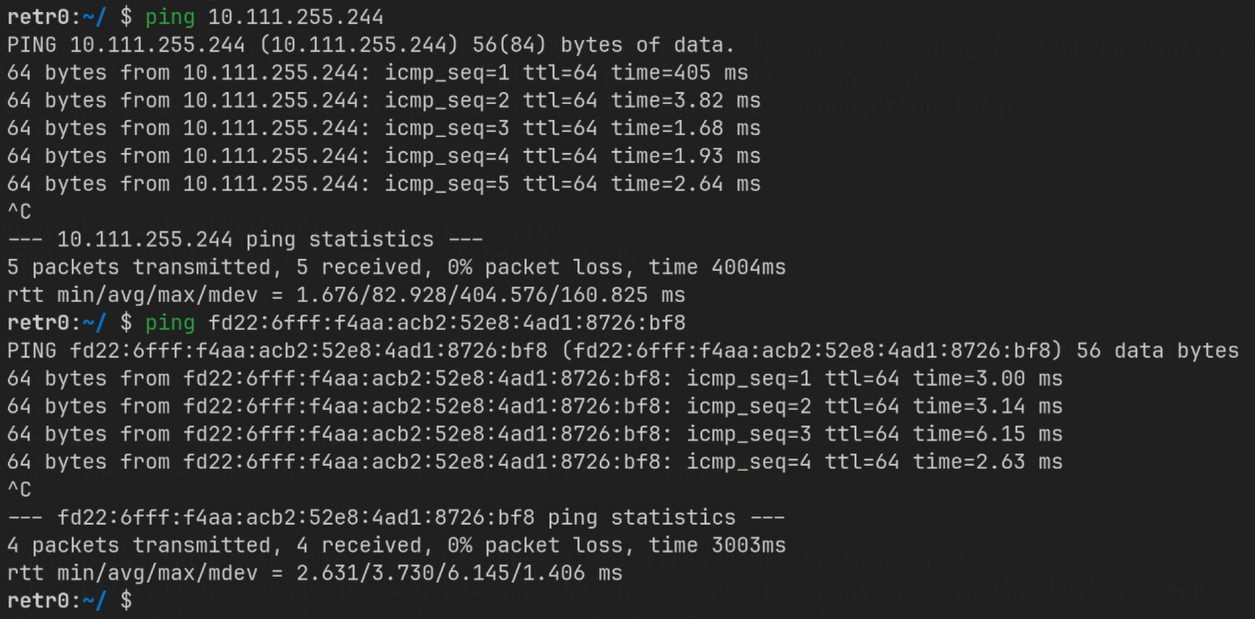
\includegraphics[width=\textwidth]{5/pinging.jpg}
  \caption{ICMP kajapäringud, mis edastati rakenduse poolt määratud IPv4 ja IPv6 aadresside abil}
\end{figure}

\newpage

Esimese paketi latentsus oli ligikaudu \emph{405 ms}, samas kui järgnevad paketid vajasid ainult ligikaudu
\emph{4 ms}. See demonstreerib, et rakendus suutis avastada kaugsõlme ning luua otsese ühenduse lühikese aja jooksul,
ilma et oleks vaja käsitsi võrgukonfiguratsiooni, näiteks
\href{https://en.wikipedia.org/wiki/Port_forwarding}{port forwarding}'ut
\footnote{\texttt{iroh} teek kasutab sisemiselt protokolle nagu
  \href{https://en.wikipedia.org/wiki/Universal_Plug_and_Play}{UPnP} ja
  \href{https://en.wikipedia.org/wiki/NAT_Port_Mapping_Protocol}{NAT-PMP},
  et automaatselt konfigureerida ruuteri pordisuunamisi juhul, kui võrgukeskkond seda toetab.}.

\subsection{Rakenduse testimine Minecrafti abil}

Rakenduse hindamiseks praktilise koormuse all testiti mitmikmängu ühenduvust
\href{https://en.wikipedia.org/wiki/Minecraft}{Minecraftis} kahe erinevates riikides paikneva sõlme vahel.
Esialgu ei suutnud sõlmed mänguühendust luua hoolimata edukast ICMP-side toimimisest.

Probleemi põhjuseks osutus ICMP \texttt{Packet Too Big} sõnumi vigane implementatsioon.
Protokolli spetsifikatsiooni kohaselt peab sõnum sisaldama osa algsest IP-paketist, et operatsioonisüsteem
saaks tuvastada mõjutatud ühenduse ning rakendada sobivat fragmenteerimiskäitumist. Pärast implementatsiooni muutmist,
et kaasata algse paketi kasulik koormus, saavutati edukalt stabiilne mitmikmängu ühendus.

\phantomsection
\section*{Kokkuvõte}
\addcontentsline{toc}{section}{Kokkuvõte}

Käesoleva töö käigus omandati teadmisi tehnikatest, mida kasutatakse otseste peer-to-peer ühenduste loomiseks kahe arvuti vahel,
sealhulgas olukordades, kus mõlemad seadmed paiknevad piiravate võrgukeskkondade taga, näiteks kodu- või kontorivõrkudes.
Projekt võimaldas uurida valdkonda, milles varasem kogemus oli piiratud, ning aitas oluliselt parandada arusaamist
alusmõistetest ja implementatsioonimeetoditest.

Pärast uurimistöö etappi viidi läbi eksperimente fundamentaalsete tehnikatega, mis on vajalikud otseste ühenduste loomiseks
Interneti kaudu arvutite vahel, mis ei ole tavapäraselt ligipääsetavad. Arendati kohandatud lahendus, et uurida meetodeid
ühenduste avastamiseks ja loomiseks suvaliste identifikaatorite abil.

Pärast edukat eksperimenteerimist põhitehnikatega arendati täielikult funktsionaalne rakendus, mis suudab toimida VPN-lahendusena,
luues otseseid ühendusi määratud sõlmede vahel \texttt{iroh} teegi abil. Teek pakub identifikaatorit, mis esindab avalikku krüpteerimisvõtit,
ning mida kasutatakse lisaks dünaamiliseks sõlmede avastamiseks ja võimalike ühendusteede määramiseks Internetis.

Valminud rakendus töötab usaldusväärselt enamikes testitud olukordades ning on loodud hooldatavust ja selgust silmas pidades tänu lihtsale koodibaasile.
Projekt demonstreerib implementeeritud lähenemise praktilist rakendatavust ka selle praeguses seisus. Tulevane töö keskendub rakenduse edasiarendamisele
ja täiustamisele isiklikuks kasutuseks ning mitmikmängu stsenaariumide jaoks.

\clearpage
\section*{Summary}
\addcontentsline{toc}{section}{Summary}

This work presents the design and implementation of \emph{petope},
a peer-to-peer VPN development project created by \theauthor to explore how two computers can be connected directly
across the Internet without requiring manual port forwarding, static public addresses, or a traditional central VPN relay.
The project was motivated by the practical difficulties of accessing self-hosted services and by the desire to understand,
in a hands-on way, how modern mesh VPN systems such as Tailscale and decentralized networking projects operate.
In addition to the technical goal, the work also aimed to produce a solution that could later be used for private remote access and multiplayer gaming.

The research phase examined several existing approaches to decentralized connectivity and peer discovery.
Particular attention was given to the limitations of conventional VPN setups, the role of NAT traversal, and the problem of
discovering peers when no central coordinator is available. Existing solutions and protocols were studied, including Tailscale, Radmin VPN, Yggdrasil,
BitTorrent-style distributed hash tables, gossip-based discovery, and the \texttt{iroh} networking library.
This research clarified the trade-offs between centralized control, usability, security, and decentralization.
It also showed that a practical VPN implementation must solve not only encryption and addressing, but also peer discovery, dynamic routing, packet delivery, and behavior behind NAT and firewalls.

On the implementation side, the project was developed in Rust and structured around a clear progression from
simple networking experiments to a complete application. The initial experiments covered UDP communication, peer discovery,
UDP hole punching, TCP hole punching attempts, and local multicast DNS discovery. These tests were used to identify what works
reliably in realistic network environments and where transport-layer limitations appear. Based on these findings,
the final application was designed to use the \texttt{iroh} library for secure peer identification, connection setup, and path negotiation.
A peer is identified by a cryptographic public key, and the application automatically derives network information from that identity,
reducing the amount of manual configuration required from the user.

The final solution includes local configuration handling, automatic generation of persistent peer keys,
virtual network interface support through a TUN device, packet routing between peers, MTU handling, and message forwarding between
the application and the operating system network stack. The implementation also includes support for reconnection and for updating peer endpoints when network conditions change.
Because VPN traffic must sometimes exceed the path MTU, the project also implements ICMP \emph{Packet Too Big} responses so that hosts can adjust packet sizes correctly.
This proved important during testing and directly affected the reliability of higher-level applications.

The completed system was evaluated through practical tests on two computers and through a multiplayer Minecraft session.
The tests showed that the application can establish a direct peer-to-peer connection after an initial relay-assisted handshake and then switch to a low-latency direct path.
In one test, the first packet experienced a noticeably higher delay, while later packets were delivered with much lower latency,
confirming that peer discovery and direct connectivity were functioning as intended.
A later Minecraft test exposed an error in the handling of ICMP fragmentation messages; after correcting this issue by including the required part of the original packet, stable game connectivity was achieved.
Overall, the work demonstrates that a functional peer-to-peer VPN can be built using existing Rust networking tools and that
the resulting system is practical for self-hosting and gaming scenarios while remaining small enough to understand and extend.


\end{document}
